\documentclass[12pt,a4paper]{article}

%% ---------- mathematics ----------
\usepackage{amsmath,amsthm,amssymb,mathtools}

%% ---------- graphics & diagrams ----------
\usepackage{tikz}
\usetikzlibrary{arrows.meta,positioning,shapes.geometric,calc,fit,backgrounds,matrix,decorations.pathreplacing}
\usepackage{graphicx}

%% ---------- tables ----------
\usepackage{booktabs,tabularx,multirow,longtable,array}

%% ---------- algorithms ----------
\usepackage[ruled,vlined,linesnumbered]{algorithm2e}

%% ---------- coloured boxes ----------
\usepackage[most]{tcolorbox}

%% ---------- hyperlinks & cross-refs ----------
\usepackage{hyperref}
\usepackage[capitalize,noabbrev]{cleveref}

%% ---------- page layout ----------
\usepackage[margin=1in]{geometry}
\usepackage{fancyhdr}
\usepackage{enumitem}
\usepackage{xcolor}

%% ---------- fonts & misc ----------
\usepackage{microtype}

%% ============================================================
%%  Custom tcolorbox environments
%% ============================================================
\newtcolorbox{keyinsight}[1][]{%
  colback=blue!5!white,colframe=blue!75!black,
  fonttitle=\bfseries,title=Key Insight,#1}

\newtcolorbox{example}[1][]{%
  colback=green!5!white,colframe=green!75!black,
  fonttitle=\bfseries,title=Example,#1}

\newtcolorbox{warningbox}[1][]{%
  colback=red!5!white,colframe=red!75!black,
  fonttitle=\bfseries,title=Warning,#1}

%% ============================================================
%%  amsthm environments
%% ============================================================
\newtheorem{theorem}{Theorem}[section]
\newtheorem{lemma}[theorem]{Lemma}
\newtheorem{definition}{Definition}[section]
\newtheorem{remark}{Remark}[section]
\newtheorem{proposition}[theorem]{Proposition}
\newtheorem{corollary}[theorem]{Corollary}

%% ============================================================
%%  Custom commands (collected from all sessions in this file)
%% ============================================================
\newcommand{\R}{\mathbb{R}}
\newcommand{\Loss}{\mathcal{L}}
\newcommand{\wh}[1]{w^{h}_{#1}}
\newcommand{\yhat}{\hat{y}}
\newcommand{\pd}[2]{\frac{\partial #1}{\partial #2}}
\newcommand{\wji}{w_{ji}^{h}}
\newcommand{\wkj}{w_{kj}}
\newcommand{\sho}{s_{j}^{h}}
\newcommand{\sko}{s_{k}^{o}}
\newcommand{\deltak}{\delta_{k}}
\newcommand{\deltajh}{\delta_{j}^{h}}
\newcommand{\xho}{x_{j}^{h}}
\newcommand{\xko}{x_{k}^{o}}
\newcommand{\ReLU}{\operatorname{ReLU}}
\newcommand{\pderiv}[2]{\dfrac{\partial #1}{\partial #2}}

\pagestyle{fancy}
\fancyhf{}
\lhead{\textsc{Deep Learning} --- IIIT Dharwad}
\rhead{Neural Networks: Feedforward, Backpropagation, and Gradient Descent}
\rfoot{Page \thepage}
\lfoot{Prof.\ S R M Prasanna \& Dr.\ Sunil Saumya}
\renewcommand{\headrulewidth}{0.4pt}

\title{%
  {\Large\bfseries Deep Learning Course}\\[6pt]
  {\LARGE Neural Networks: Feedforward, Backpropagation, and Gradient Descent}\\[4pt]
  {\normalsize IIIT Dharwad --- M.Tech Programme}
}
\author{Prof.\ S R M Prasanna \& Dr.\ Sunil Saumya}
\date{Sessions 5, 6, 7}

\begin{document}

\maketitle
\tableofcontents
\clearpage

%% ============================================================
%% Session 05: Neural Network: Feedforward and Backpropagation
%% ============================================================
\part{Session 05: Neural Network: Feedforward and Backpropagation}

% ════════════════════════════════════════════════════════════════════════════
%  TITLE PAGE
% ════════════════════════════════════════════════════════════════════════════
\begin{titlepage}
  \centering
  \vspace*{2cm}

  {\LARGE\bfseries Deep Learning Course\\[0.4em]
   \rule{\linewidth}{0.5pt}\\[0.6em]
   Session 05: Neural Network\\Feedforward and Backpropagation\\
   \rule{\linewidth}{0.5pt}}

  \vspace{1.5cm}

  \begin{tcolorbox}[colback=blue!5!white,colframe=blue!50!black,width=0.85\linewidth]
    \centering
    \begin{tabular}{ll}
      \textbf{Session Number:} & 05 \\[4pt]
      \textbf{Topic:}          & Multi-layer feedforward networks, differentiable \\
                               & activation functions, backpropagation, chain rule \\[4pt]
      \textbf{Deck:}           & \texttt{03-DL-NeuralNetworkIntroduction} \\[4pt]
      \textbf{Instructors:}    & Prof.\ S~R~M~Prasanna \& Dr.\ Sunil Saumya \\[4pt]
      \textbf{Institution:}    & Dept.\ of Data Science \& Artificial Intelligence \\
                               & Indian Institute of Information Technology Dharwad \\[4pt]
      \textbf{Duration:}       & 1 hour 51 minutes 36 seconds \\[4pt]
      \textbf{Video:}          & \url{https://vimeo.com/1142296251} \\
    \end{tabular}
  \end{tcolorbox}

  \vspace{1.5cm}

  \begin{abstract}
    \noindent
    Session~05 extends the single-layer perceptron framework to
    \emph{multi-layer feedforward neural networks} (MLFFNNs).  The session
    opens with a recap of why linearly non-separable problems require hidden
    layers, then identifies the \emph{hard learning problem}: the perceptron
    learning rule cannot be applied to hidden-layer weights because no target
    output is available there.  The resolution is replacing the
    non-differentiable step function with \emph{differentiable sigmoidal
    activations} (logistic and hyperbolic tangent), enabling the
    \emph{backpropagation algorithm} (generalised delta rule) to propagate
    error gradients from the output layer back through every hidden layer via
    the chain rule.  A complete numerical forward pass on an IQ/CGPA
    prediction example (ReLU hidden activations, linear output) is worked
    through, followed by the derivation of the first backpropagation
    gradients $\partial\Loss/\partial v_1$, $\partial\Loss/\partial v_2$, and
    $\partial\Loss/\partial b_3$.
  \end{abstract}

  \vfill
  {\small Notes compiled from lecture transcript and slide visual extractions.\\
   Reference textbook: B.~Yegnanarayana, \emph{Artificial Neural Networks},
   PHI, New Delhi, 1999.}
\end{titlepage}

% ════════════════════════════════════════════════════════════════════════════
%  TABLE OF CONTENTS
% ════════════════════════════════════════════════════════════════════════════

\newpage

% ════════════════════════════════════════════════════════════════════════════
%  1. INTRODUCTION
% ════════════════════════════════════════════════════════════════════════════
\section{Introduction}
\label{sec:intro}

The single-layer perceptron, equipped with a step (hard-limiting) output
function, can learn any \emph{linearly separable} classification boundary.
However, a vast class of real-world problems---from XOR-type logical functions
to complex regression tasks---requires non-linear decision surfaces.
Session~04 established that adding more layers of perceptrons can, in
principle, represent arbitrary convex (two layers) or non-convex (three
layers) decision regions.  Session~05 confronts the natural follow-up
question: \emph{how do we train such a multi-layer network?}

The answer unfolds in two conceptual steps.
\begin{enumerate}[label=\textbf{Step \arabic*.},leftmargin=3em]
  \item \textbf{Identify the obstacle.}  In a multi-layer network only the
    output-layer activations are directly observable; the hidden-layer target
    outputs are \emph{unknown}.  Without a target, the simple
    error $= \text{target} - \text{actual}$ cannot be formed at hidden nodes,
    so the perceptron learning rule breaks down.  Prof.~Prasanna terms this
    the \emph{hard learning problem}.

  \item \textbf{Resolve it with differentiable activations and the chain
    rule.}  Replacing the step function with smooth sigmoidal functions
    (logistic or hyperbolic tangent) makes every output differentiable.  This
    allows the output-layer error to be \emph{propagated backwards} layer by
    layer through the chain rule---the celebrated
    \emph{backpropagation algorithm}, also known as the
    \emph{generalised delta rule}.
\end{enumerate}

The session then walks through a concrete numerical example: a two-input
(IQ, CGPA) network with one hidden layer of two ReLU neurons and a linear
output neuron predicting a student's salary package.

\begin{keyinsight}[title=Session~05 in One Sentence]
  Backpropagation solves the hard learning problem by using differentiable
  activation functions and the chain rule to express hidden-layer errors in
  terms of the observable output-layer error, enabling gradient descent over
  \emph{all} network weights simultaneously.
\end{keyinsight}

% ════════════════════════════════════════════════════════════════════════════
%  2. BACKGROUND AND PREREQUISITES
% ════════════════════════════════════════════════════════════════════════════
\section{Background and Prerequisites}
\label{sec:background}

\subsection{The Perceptron and its Limitations}
\label{subsec:perceptron}

A single perceptron computes a weighted sum of its inputs followed by a
hard-limiting (step) output function.  For an input vector
$\mathbf{a} = (a_1, \ldots, a_I)^{\top}$ and weight vector $\mathbf{w}$, the
perceptron output is
\begin{equation}
  s = \operatorname{sgn}\!\left(\mathbf{w}^{\top}\mathbf{a} - \theta\right),
  \qquad \operatorname{sgn}(x) =
  \begin{cases} +1 & x \geq 0, \\ -1 & x < 0. \end{cases}
  \label{eq:perceptron}
\end{equation}
The \emph{perceptron learning rule} updates weights as
\begin{equation}
  \Delta \mathbf{w} = \eta\,\delta\,\mathbf{a},
  \qquad \delta = b - \operatorname{sgn}(\mathbf{w}^{\top}\mathbf{a}),
  \label{eq:percep-learning}
\end{equation}
where $b$ is the desired (target) output and $\eta > 0$ is the learning rate.
This rule requires a \emph{known target} at every neuron; a requirement
impossible to satisfy for hidden layers.

\subsection{Representing Nonlinear Decision Regions}
\label{subsec:nonlinear}

\begin{definition}[Convex and Non-convex Problems]
  \label{def:convex}
  A classification problem is \emph{convex} if the decision region of every
  class is a convex set.  It is \emph{non-convex} otherwise.
\end{definition}

The architectural depth required scales with the complexity of the desired
boundary:
\begin{itemize}
  \item \textbf{Linearly separable:} 1 layer (input + output perceptron).
  \item \textbf{Convex non-linear:} 2 layers (input + 1 hidden + output).
  \item \textbf{Non-convex:} 3 layers (input + 2 hidden + output).
\end{itemize}

While this representational hierarchy was understood, \emph{training} these
deeper networks remained an open problem for nearly a decade---the neural
network field stalled until the backpropagation algorithm provided a
practical solution.

\subsection{Supervised Learning Setup}
\label{subsec:supervised}

Throughout this session the learning task is \emph{supervised}: given a
dataset $\{(\mathbf{a}(m), \mathbf{b}(m))\}_{m=1}^{M}$ of input--output
pairs, the goal is to find weights such that for each pattern $m$ the network
output $\mathbf{b}'(m)$ approximates the desired output $\mathbf{b}(m)$ with
small error.  The squared error for pattern $m$ is
\begin{equation}
  E(m) = \frac{1}{2}\sum_{k=1}^{K}\bigl[b_k(m) - b'_k(m)\bigr]^2,
  \label{eq:error}
\end{equation}
where $K$ is the number of output units.  The factor of $\tfrac{1}{2}$ is
conventional and simplifies later derivatives.

% ════════════════════════════════════════════════════════════════════════════
%  3. THREE-LAYER FEEDFORWARD NETWORK
% ════════════════════════════════════════════════════════════════════════════
\section{The Three-Layer Feedforward Neural Network}
\label{sec:architecture}

\subsection{Network Notation (Figure 4.12)}
\label{subsec:notation}

Following Yegnanarayana (1999), the canonical three-layer network (called a
\emph{two-layer perceptron} in that text because the linear input layer is not
counted as a ``learning'' layer) has the following structure.

\begin{definition}[Three-Layer MLFFNN]
  \label{def:threelayer}
  A three-layer multi-layer feedforward neural network (MLFFNN) consists of:
  \begin{itemize}
    \item \textbf{Input layer}: $I$ linear units indexed by $i = 1,\ldots,I$,
      with activations $a_i$.
    \item \textbf{Hidden layer}: $J$ nonlinear units indexed by $j = 1,\ldots,J$,
      with outputs $s_j^h$.
    \item \textbf{Output layer}: $K$ nonlinear units indexed by $k = 1,\ldots,K$,
      with outputs $s_k^o$.
  \end{itemize}
  Weights from input unit $i$ to hidden unit $j$ are denoted $w_{ji}^h$.
  Weights from hidden unit $j$ to output unit $k$ are denoted $w_{kj}$.
\end{definition}

The superscript $h$ on input-to-hidden weights is purely notational---it
distinguishes the two sets of weights and is dropped for the hidden-to-output
set.

\subsection{TikZ Diagram: Three-Layer FFNN Architecture}
\label{subsec:arch-tikz}

\cref{fig:threelayer} shows the fully-connected three-layer architecture.

\begin{figure}[htbp]
\centering
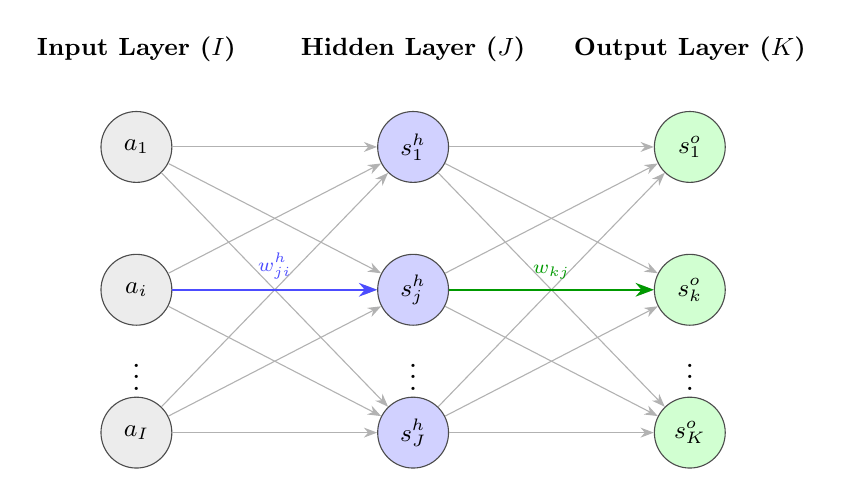
\begin{tikzpicture}[
    node distance=1.6cm and 2.6cm,
    neuron/.style={circle, draw=black!70, fill=white, minimum size=0.9cm,
                   font=\small},
    inputn/.style={neuron, fill=gray!15},
    hiddenn/.style={neuron, fill=blue!18},
    outputn/.style={neuron, fill=green!18},
    bias/.style={rectangle, draw=black!50, fill=yellow!20, minimum size=0.7cm,
                 font=\scriptsize},
    >=Stealth
  ]

  %% Input layer
  \node[inputn] (i1) {$a_1$};
  \node[inputn, below=0.9cm of i1] (i2) {$a_i$};
  \node[inputn, below=0.9cm of i2] (i3) {$a_I$};

  %% Hidden layer
  \node[hiddenn, right=2.6cm of i1] (h1) {$s_1^h$};
  \node[hiddenn, below=0.9cm of h1] (h2) {$s_j^h$};
  \node[hiddenn, below=0.9cm of h2] (h3) {$s_J^h$};

  %% Output layer
  \node[outputn, right=2.6cm of h1] (o1) {$s_1^o$};
  \node[outputn, below=0.9cm of o1] (o2) {$s_k^o$};
  \node[outputn, below=0.9cm of o2] (o3) {$s_K^o$};

  %% Input → Hidden (selected edges)
  \foreach \src in {i1,i2,i3}{
    \foreach \dst in {h1,h2,h3}{
      \draw[->, gray!60, thin] (\src) -- (\dst);
    }
  }

  %% Annotate one weight
  \draw[->, blue!70, thick] (i2) -- node[above, sloped, font=\scriptsize]
        {$w_{ji}^h$} (h2);

  %% Hidden → Output (selected edges)
  \foreach \src in {h1,h2,h3}{
    \foreach \dst in {o1,o2,o3}{
      \draw[->, gray!60, thin] (\src) -- (\dst);
    }
  }

  %% Annotate one weight
  \draw[->, green!60!black, thick] (h2) -- node[above, sloped, font=\scriptsize]
        {$w_{kj}$} (o2);

  %% Layer labels
  \node[above=0.5cm of i1, font=\bfseries\small] {Input Layer ($I$)};
  \node[above=0.5cm of h1, font=\bfseries\small] {Hidden Layer ($J$)};
  \node[above=0.5cm of o1, font=\bfseries\small] {Output Layer ($K$)};

  %% Vertical dots
  \node[font=\large] at ($(i2)!0.5!(i3) + (0,-0.1cm)$) {$\vdots$};
  \node[font=\large] at ($(h2)!0.5!(h3) + (0,-0.1cm)$) {$\vdots$};
  \node[font=\large] at ($(o2)!0.5!(o3) + (0,-0.1cm)$) {$\vdots$};

\end{tikzpicture}
\caption{Three-layer multi-layer feedforward neural network (Figure~4.12 from
  Yegnanarayana, 1999).  The input layer is linear; the hidden and output
  layers are nonlinear.  Every input unit connects to every hidden unit
  (weights $w_{ji}^h$), and every hidden unit connects to every output unit
  (weights $w_{kj}$).}
\label{fig:threelayer}
\end{figure}

\subsection{Forward Propagation Equations}
\label{subsec:forward-eqs}

The computation for each layer proceeds as a two-step process: a linear
\emph{weighted summation} followed by a nonlinear \emph{activation function}.

\paragraph{Hidden layer.}
For hidden unit $j$:
\begin{align}
  x_j^h &= \sum_{i=1}^{I} w_{ji}^h\, a_i + b_j^h,
  \label{eq:hidden-net} \\
  s_j^h &= f\!\left(x_j^h\right),
  \label{eq:hidden-act}
\end{align}
where $b_j^h$ is the bias of hidden unit $j$ and $f(\cdot)$ is the
differentiable activation function.

\paragraph{Output layer.}
For output unit $k$:
\begin{align}
  x_k^o &= \sum_{j=1}^{J} w_{kj}\, s_j^h + b_k^o,
  \label{eq:output-net} \\
  s_k^o &= f\!\left(x_k^o\right).
  \label{eq:output-act}
\end{align}

\begin{keyinsight}[title=Why ``Feedforward''?]
  Information flows strictly from left (input) to right (output): input
  activations $\to$ hidden layer $\to$ output layer.  There are no feedback
  connections during inference.  The name \emph{feedforward} reflects this
  unidirectional signal flow.
\end{keyinsight}

% ════════════════════════════════════════════════════════════════════════════
%  4. DIFFERENTIABLE ACTIVATION FUNCTIONS
% ════════════════════════════════════════════════════════════════════════════
\section{Differentiable Activation Functions}
\label{sec:activations}

\subsection{Why Differentiability Matters}
\label{subsec:why-diff}

The step function used in the classical perceptron is:
\begin{equation}
  f_{\mathrm{step}}(x) = \begin{cases} 1 & x \geq 0, \\ 0 & x < 0. \end{cases}
  \label{eq:step}
\end{equation}
Its derivative is zero everywhere except at $x=0$, where it is undefined.
This means that $\partial E / \partial w_{ji}^h$ involves $f'(x_j^h) = 0$
for all $x_j^h \neq 0$, killing any gradient signal that would adjust hidden
weights.  The backpropagation algorithm requires \emph{non-zero} derivatives
throughout.

\begin{warningbox}[title=The Step Function Cannot be Used in Hidden Layers]
  If $f$ is the step function, then $f'(x) = 0$ almost everywhere.  The
  gradient $\partial E / \partial w_{ji}^h$ evaluates to zero regardless of
  the error, making it \emph{impossible} to update input-to-hidden weights via
  gradient descent.  This is the root cause of the ``hard learning problem''.
\end{warningbox}

\subsection{The Logistic (Sigmoid) Function}
\label{subsec:logistic}

The logistic function with slope parameter $\beta > 0$ is:
\begin{equation}
  f(x) = \frac{1}{1 + \exp(-2\beta x)},
  \qquad f(x) \in (0, 1).
  \label{eq:logistic}
\end{equation}
Its derivative has a convenient closed form:
\begin{equation}
  \dot{f}(x) = 2\beta\, f(x)\bigl(1 - f(x)\bigr).
  \label{eq:logistic-deriv}
\end{equation}
Key values: $f(0) = 0.5$; $f(x) \to 1$ as $x \to +\infty$; $f(x) \to 0$
as $x \to -\infty$.

\begin{remark}
  The standard logistic sigmoid $\sigma(x) = (1+e^{-x})^{-1}$ is a special
  case of \cref{eq:logistic} with $\beta = \tfrac{1}{2}$, giving
  $\dot{\sigma}(x) = \sigma(x)(1-\sigma(x))$.
\end{remark}

\subsection{The Hyperbolic Tangent Function}
\label{subsec:tanh}

The hyperbolic tangent activation is:
\begin{equation}
  f(x) = \tanh(\beta x) = \frac{e^{\beta x} - e^{-\beta x}}{e^{\beta x} + e^{-\beta x}},
  \qquad f(x) \in (-1, 1).
  \label{eq:tanh}
\end{equation}
Its derivative is:
\begin{equation}
  \dot{f}(x) = \beta\bigl(1 - f^2(x)\bigr).
  \label{eq:tanh-deriv}
\end{equation}
The symmetric range $(-1,+1)$ often leads to faster convergence than logistic
because the mean activation is centred at zero, reducing the covariate shift
between layers.

\subsection{The ReLU Function}
\label{subsec:relu}

Modern deep networks frequently use the Rectified Linear Unit (ReLU):
\begin{equation}
  f(x) = \max(0, x),
  \qquad \dot{f}(x) = \begin{cases} 1 & x > 0, \\ 0 & x \leq 0. \end{cases}
  \label{eq:relu}
\end{equation}
ReLU does not saturate for positive inputs (unlike sigmoid/tanh), avoiding
the vanishing gradient problem in deeper architectures.  In this session's
numerical example, ReLU is used in the hidden layer while the output layer
uses a \emph{linear} (identity) activation for regression.

\subsection{Comparison Table}
\label{subsec:activation-table}

\cref{tab:activations} summarises the four activation functions encountered in
this session.

\begin{table}[htbp]
\centering
\caption{Summary of activation functions.  $\beta$ is a slope parameter
  (default $\beta = 0.5$ for logistic and tanh).}
\label{tab:activations}
\renewcommand{\arraystretch}{1.4}
\begin{tabularx}{\linewidth}{lXXXX}
\toprule
\textbf{Function} & \textbf{Formula} & \textbf{Derivative} & \textbf{Range}
  & \textbf{Typical Use} \\
\midrule
Step (hard limiting)
  & $\mathbf{1}[x \geq 0]$
  & $0$ (a.e.)
  & $\{0,1\}$
  & Output of classical perceptron only \\
Logistic (sigmoid)
  & $\frac{1}{1+e^{-2\beta x}}$
  & $2\beta f(1-f)$
  & $(0,1)$
  & Hidden/output layers (binary classification) \\
Tanh
  & $\tanh(\beta x)$
  & $\beta(1-f^2)$
  & $(-1,1)$
  & Hidden layers (zero-centred) \\
ReLU
  & $\max(0,x)$
  & $\mathbf{1}[x>0]$
  & $[0,\infty)$
  & Hidden layers in deep networks \\
\bottomrule
\end{tabularx}
\end{table}

% ════════════════════════════════════════════════════════════════════════════
%  5. BACKPROPAGATION: THE GENERALISED DELTA RULE
% ════════════════════════════════════════════════════════════════════════════
\section{Backpropagation: The Generalised Delta Rule}
\label{sec:backprop}

\subsection{Gradient Descent on the Error Surface}
\label{subsec:grad-descent}

Backpropagation is a \emph{gradient descent} algorithm.  The error $E(m)$
defined in \cref{eq:error} is a surface in the space of all weights.  The
goal is to find the weight configuration that corresponds to a (local) minimum
of this surface.  Moving in the direction of steepest descent requires
computing the gradient $\nabla_{\mathbf{w}} E$.

The weight update rule for any weight $w_{ij}$ is:
\begin{equation}
  \Delta w_{ij} = -\eta\,\frac{\partial E(m)}{\partial w_{ij}},
  \qquad \eta > 0,
  \label{eq:grad-descent}
\end{equation}
\begin{equation}
  w_{ij}(m+1) = w_{ij}(m) + \Delta w_{ij}.
  \label{eq:weight-update}
\end{equation}
The negative sign ensures movement \emph{downhill} on the error surface.

\subsection{The Hard Learning Problem Revisited}
\label{subsec:hard-learning}

For output-layer weights $w_{kj}$, computing $\partial E / \partial w_{kj}$
is straightforward because the error $E(m)$ depends directly on the
output-layer activations $s_k^o$.  For hidden-layer weights $w_{ji}^h$,
however, $E(m)$ depends on $w_{ji}^h$ only \emph{indirectly}, through
$s_j^h \to s_k^o$.  The chain rule bridges this gap.

\begin{keyinsight}[title=The Core Idea of Backpropagation]
  Even though no target is available at hidden units, the error computed at
  the output layer can be \emph{mathematically expressed} in terms of
  hidden-layer outputs, provided those outputs are produced by a differentiable
  activation function.  The chain rule then gives a closed-form gradient for
  every weight in the network.
\end{keyinsight}

\subsection{Deriving the Output-Layer Gradient}
\label{subsec:output-gradient}

For output unit $k$ with net input $x_k^o = \sum_j w_{kj} s_j^h + b_k^o$:
\begin{align}
  \frac{\partial E}{\partial w_{kj}}
    &= \frac{\partial E}{\partial s_k^o}
       \cdot\frac{\partial s_k^o}{\partial x_k^o}
       \cdot\frac{\partial x_k^o}{\partial w_{kj}} \notag \\[4pt]
    &= \bigl[-(b_k - s_k^o)\bigr]
       \cdot \dot{f}(x_k^o)
       \cdot s_j^h.
  \label{eq:output-grad}
\end{align}
Defining the \emph{output delta}:
\begin{equation}
  \delta_k^o = (b_k - s_k^o)\,\dot{f}(x_k^o),
  \label{eq:delta-output}
\end{equation}
the update becomes $\Delta w_{kj} = \eta\,\delta_k^o\,s_j^h$.

\subsection{Deriving the Hidden-Layer Gradient}
\label{subsec:hidden-gradient}

For hidden unit $j$ with net input $x_j^h = \sum_i w_{ji}^h\,a_i + b_j^h$:
\begin{align}
  \frac{\partial E}{\partial w_{ji}^h}
    &= \sum_{k=1}^{K}
       \frac{\partial E}{\partial s_k^o}
       \cdot\frac{\partial s_k^o}{\partial x_k^o}
       \cdot\frac{\partial x_k^o}{\partial s_j^h}
       \cdot\frac{\partial s_j^h}{\partial x_j^h}
       \cdot\frac{\partial x_j^h}{\partial w_{ji}^h} \notag \\[4pt]
    &= \dot{f}(x_j^h)
       \left[\sum_{k=1}^{K} \delta_k^o\,w_{kj}\right]
       \cdot a_i.
  \label{eq:hidden-grad}
\end{align}
Defining the \emph{hidden delta} as:
\begin{equation}
  \delta_j^h = \dot{f}(x_j^h)\sum_{k=1}^{K}\delta_k^o\,w_{kj},
  \label{eq:delta-hidden}
\end{equation}
the update rule for hidden-layer weights is $\Delta w_{ji}^h = \eta\,\delta_j^h\,a_i$.

\begin{remark}
  The hidden delta $\delta_j^h$ in \cref{eq:delta-hidden} is a weighted sum of
  \emph{output deltas} $\delta_k^o$, propagated back through the weights
  $w_{kj}$ and modulated by the local derivative $\dot{f}(x_j^h)$.  This is
  why the algorithm is called \emph{back}propagation: the error signal travels
  from output to input.
\end{remark}

\subsection{Comparison: Discrete vs.\ Continuous Delta Rule}
\label{subsec:discrete-vs-continuous}

\cref{tab:delta-rules} contrasts the classical (discrete) perceptron learning
law with the generalised (continuous/differentiable) delta rule.

\begin{table}[htbp]
\centering
\caption{Discrete perceptron learning law vs.\ generalised delta rule.}
\label{tab:delta-rules}
\renewcommand{\arraystretch}{1.5}
\begin{tabularx}{\linewidth}{lXX}
\toprule
\textbf{Property} & \textbf{Discrete (Perceptron)} & \textbf{Generalised Delta Rule} \\
\midrule
Output function $f$
  & Step / signum (non-differentiable)
  & Sigmoid, tanh, ReLU (differentiable) \\
Weight update rule
  & $\Delta w = \eta\,(b - \operatorname{sgn}(\mathbf{w}^{\top}\mathbf{a}))\,\mathbf{a}$
  & $\Delta w_{ij} = -\eta\,\partial E/\partial w_{ij}$ \\
Applicable to
  & Output layer only (target known)
  & All layers (chain rule handles hidden layers) \\
Error definition
  & Direct: $\delta = b - s$
  & Gradient: $\partial E / \partial w$ via chain rule \\
Key innovation
  & $\delta$ proportional to error $b - s$
  & $\delta$ proportional to error \emph{times} $\dot{f}(x)$ \\
Convergence
  & Guaranteed (linearly separable data)
  & Convergence to local minimum (not guaranteed globally) \\
\bottomrule
\end{tabularx}
\end{table}

% ════════════════════════════════════════════════════════════════════════════
%  6. THE TRAINING LOOP
% ════════════════════════════════════════════════════════════════════════════
\section{The Neural Network Training Loop}
\label{sec:training-loop}

\subsection{Forward and Backward Passes}
\label{subsec:fwd-bwd}

Training a neural network alternates between two phases in every iteration
(epoch/mini-batch):

\begin{enumerate}[label=\textbf{Phase \arabic*.}]
  \item \textbf{Forward Pass.} Feed the input through the network
    layer-by-layer to obtain the prediction $\yhat$.
  \item \textbf{Loss Computation.} Compute the scalar loss
    $\Loss(\yhat, y)$.
  \item \textbf{Backward Pass.} Use the chain rule to compute
    $\partial\Loss/\partial w$ for every weight $w$ in the network.
  \item \textbf{Parameter Update.} Update all weights using the gradient
    descent rule of \cref{eq:weight-update}.
\end{enumerate}

\cref{fig:training-loop} illustrates this iterative cycle.

\begin{figure}[htbp]
\centering
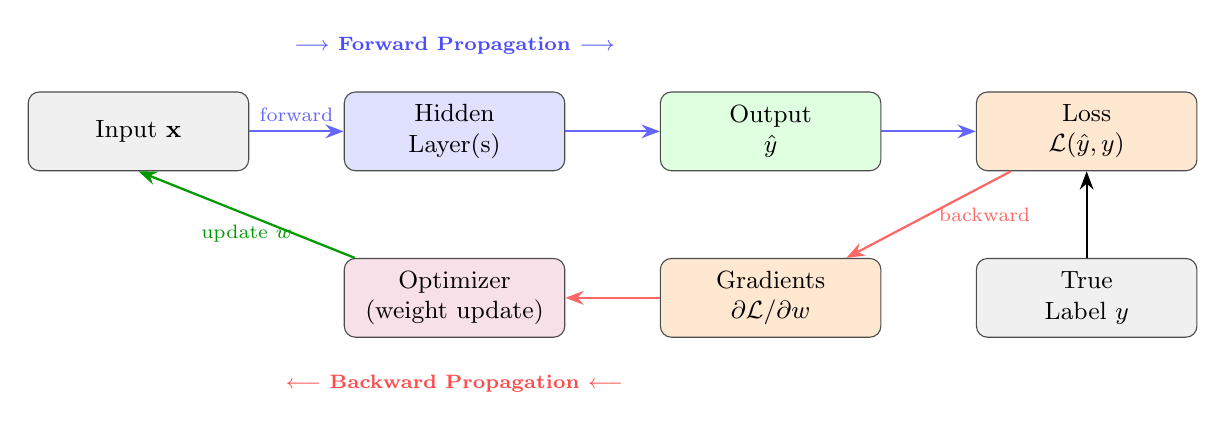
\begin{tikzpicture}[
    box/.style={rectangle, draw=black!70, rounded corners=4pt,
                minimum width=2.8cm, minimum height=1.0cm,
                align=center, font=\small, fill=white},
    inputbox/.style={box, fill=gray!12},
    hidbox/.style={box, fill=blue!12},
    outbox/.style={box, fill=green!12},
    lossbox/.style={box, fill=orange!18},
    optbox/.style={box, fill=purple!12},
    >=Stealth,
    node distance=1.2cm and 0.8cm
  ]

  %% Forward pass nodes (top row, left to right)
  \node[inputbox] (input) {Input $\mathbf{x}$};
  \node[hidbox, right=1.2cm of input] (hidden1) {Hidden\\Layer(s)};
  \node[outbox, right=1.2cm of hidden1] (output) {Output\\$\yhat$};
  \node[lossbox, right=1.2cm of output] (loss) {Loss\\$\Loss(\yhat, y)$};

  %% True label node
  \node[inputbox, below=1.1cm of loss] (true) {True\\Label $y$};

  %% Optimizer node
  \node[optbox, below=1.1cm of hidden1] (optim) {Optimizer\\(weight update)};

  %% Gradient node
  \node[lossbox, below=1.1cm of output] (grads) {Gradients\\$\partial\Loss/\partial w$};

  %% Forward arrows
  \draw[->, thick, blue!60] (input) -- node[above, font=\scriptsize]{forward} (hidden1);
  \draw[->, thick, blue!60] (hidden1) -- (output);
  \draw[->, thick, blue!60] (output) -- (loss);
  \draw[->, thick] (true) -- (loss);

  %% Backward arrows
  \draw[->, thick, red!60] (loss) -- node[right, font=\scriptsize]{backward} (grads);
  \draw[->, thick, red!60] (grads) -- (optim);
  \draw[->, thick, green!60!black] (optim) --
        node[below, font=\scriptsize]{update $w$} (input.south);

  %% Labels
  \node[above=0.35cm of hidden1, font=\bfseries\scriptsize, blue!70]
        {$\longrightarrow$ Forward Propagation $\longrightarrow$};
  \node[below=0.35cm of optim, font=\bfseries\scriptsize, red!70]
        {$\longleftarrow$ Backward Propagation $\longleftarrow$};

\end{tikzpicture}
\caption{The neural network training loop.  In every iteration the forward
  pass computes predictions, the loss is evaluated, gradients are
  back-propagated, and the optimizer updates all weights.  This cycle repeats
  until the loss is minimised.}
\label{fig:training-loop}
\end{figure}

\subsection{Backpropagation Algorithm}
\label{subsec:bp-algo}

\cref{alg:backprop} gives the complete single-pattern backpropagation
procedure for a three-layer network.

\begin{algorithm}[htbp]
\DontPrintSemicolon
\caption{Backpropagation for a Three-Layer MLFFNN (single pattern)}
\label{alg:backprop}
\KwIn{Input $\mathbf{a}$, desired output $\mathbf{b}$, learning rate $\eta$,
      weights $\{w_{ji}^h\}$ and $\{w_{kj}\}$, biases $\{b_j^h\}$ and $\{b_k^o\}$}
\KwOut{Updated weights and biases}
\BlankLine
\tcp{--- Forward Pass ---}
\For{$j = 1$ \KwTo $J$}{
  $x_j^h \leftarrow \sum_{i} w_{ji}^h\,a_i + b_j^h$\;
  $s_j^h \leftarrow f(x_j^h)$\;
}
\For{$k = 1$ \KwTo $K$}{
  $x_k^o \leftarrow \sum_{j} w_{kj}\,s_j^h + b_k^o$\;
  $s_k^o \leftarrow f(x_k^o)$\;
}
\BlankLine
\tcp{--- Compute Loss ---}
$E \leftarrow \frac{1}{2}\sum_{k}(b_k - s_k^o)^2$\;
\BlankLine
\tcp{--- Backward Pass: Output Layer Deltas ---}
\For{$k = 1$ \KwTo $K$}{
  $\delta_k^o \leftarrow (b_k - s_k^o)\,\dot{f}(x_k^o)$\;
}
\BlankLine
\tcp{--- Backward Pass: Hidden Layer Deltas ---}
\For{$j = 1$ \KwTo $J$}{
  $\delta_j^h \leftarrow \dot{f}(x_j^h)\,\sum_{k} \delta_k^o\,w_{kj}$\;
}
\BlankLine
\tcp{--- Weight Updates ---}
\For{$k = 1$ \KwTo $K$}{
  \For{$j = 1$ \KwTo $J$}{
    $w_{kj} \leftarrow w_{kj} + \eta\,\delta_k^o\,s_j^h$\;
  }
  $b_k^o \leftarrow b_k^o + \eta\,\delta_k^o$\;
}
\For{$j = 1$ \KwTo $J$}{
  \For{$i = 1$ \KwTo $I$}{
    $w_{ji}^h \leftarrow w_{ji}^h + \eta\,\delta_j^h\,a_i$\;
  }
  $b_j^h \leftarrow b_j^h + \eta\,\delta_j^h$\;
}
\Return{Updated weights and biases}\;
\end{algorithm}

\begin{keyinsight}[title=Computational Complexity]
  Each forward pass requires $O(I \cdot J + J \cdot K)$ multiplications.
  The backward pass has the same order of complexity.  Training thus scales
  linearly in the number of parameters---a key reason backpropagation is
  computationally feasible even for large networks.
\end{keyinsight}

% ════════════════════════════════════════════════════════════════════════════
%  7. NUMERICAL EXAMPLE
% ════════════════════════════════════════════════════════════════════════════
\section{Numerical Example: IQ/CGPA to Salary Prediction}
\label{sec:example}

Dr.~Sunil Saumya walks through a concrete one-iteration example.
The problem is a regression task: predict a student's salary package (LPA)
from their IQ score and CGPA.

\subsection{Network Architecture}
\label{subsec:example-arch}

The network has:
\begin{itemize}
  \item Two real-valued inputs: $x_1 = \text{IQ}$ and $x_2 = \text{CGPA}$.
  \item One hidden layer with two neurons ($h_1$, $h_2$), each using
    \textbf{ReLU} activation.
  \item One output neuron ($\yhat$) using \textbf{linear} (identity) activation.
  \item Bias nodes: $b_1 = b_2 = b_3 = 1$.
\end{itemize}

\subsection{Weights and Data}
\label{subsec:example-weights}

The initial weights are:
\begin{align}
  w_{11} &= 0.02, & w_{12} &= 0.50, \notag \\
  w_{21} &= 0.04, & w_{22} &= -0.30, \notag \\
  v_1    &= 1.20, & v_2    &= 0.80.
  \label{eq:init-weights}
\end{align}
The first training data point is:
\begin{equation}
  x_1 = 80 \;\text{(IQ)}, \quad x_2 = 8 \;\text{(CGPA)}, \quad y = 3 \;\text{(LPA)}.
  \label{eq:data-point}
\end{equation}

\subsection{Forward Pass}
\label{subsec:forward-pass}

\paragraph{Hidden neuron $h_1$.}
\begin{align}
  z_1 &= w_{11}x_1 + w_{12}x_2 + b_1 \notag \\
      &= 0.02 \times 80 + 0.50 \times 8 + 1 \notag \\
      &= 1.60 + 4.00 + 1.00 = 6.60, \\
  h_1 &= \mathrm{ReLU}(z_1) = \max(0,\;6.60) = \mathbf{6.60}.
  \label{eq:h1}
\end{align}

\paragraph{Hidden neuron $h_2$.}
\begin{align}
  z_2 &= w_{21}x_1 + w_{22}x_2 + b_2 \notag \\
      &= 0.04 \times 80 + (-0.30) \times 8 + 1 \notag \\
      &= 3.20 - 2.40 + 1.00 = 1.80, \\
  h_2 &= \mathrm{ReLU}(z_2) = \max(0,\;1.80) = \mathbf{1.80}.
  \label{eq:h2}
\end{align}

\paragraph{Output neuron (linear activation).}
\begin{align}
  \yhat &= v_1 h_1 + v_2 h_2 + b_3 \notag \\
        &= 1.20 \times 6.60 + 0.80 \times 1.80 + 1 \notag \\
        &= 7.92 + 1.44 + 1.00 = \mathbf{10.36}.
  \label{eq:yhat}
\end{align}

\begin{example}[title=Forward Pass Summary]
  \begin{center}
  \renewcommand{\arraystretch}{1.3}
  \begin{tabular}{lll}
    \toprule
    \textbf{Quantity} & \textbf{Value} & \textbf{Remark} \\
    \midrule
    $z_1 = w_{11}x_1 + w_{12}x_2 + b_1$ & $6.60$ & Pre-activation, $h_1$ \\
    $h_1 = \mathrm{ReLU}(z_1)$           & $6.60$ & Positive, so passes through \\
    $z_2 = w_{21}x_1 + w_{22}x_2 + b_2$ & $1.80$ & Pre-activation, $h_2$ \\
    $h_2 = \mathrm{ReLU}(z_2)$           & $1.80$ & Positive, so passes through \\
    $\yhat = v_1h_1 + v_2h_2 + b_3$      & $10.36$ & Network prediction \\
    $y$                                   & $3.00$  & True label \\
    $\Loss = (y - \yhat)^2$               & $54.15$ & Very high; weights need updating \\
    \bottomrule
  \end{tabular}
  \end{center}
\end{example}

\subsection{Loss Computation}
\label{subsec:loss}

Using squared-error loss:
\begin{align}
  \Loss &= (y - \yhat)^2 = (3 - 10.36)^2 = (-7.36)^2 = 54.17.
  \label{eq:loss-val}
\end{align}

The loss of $54.17$ is very large (the best possible is $0$), indicating that
the randomly initialised weights are far from optimal.  Backpropagation will
now compute how each weight contributed to this loss and update them
accordingly.

\subsection{Backward Pass: Output-Layer Gradients}
\label{subsec:backward-pass}

The loss function and its derivative with respect to $\yhat$ are:
\begin{align}
  \Loss &= (y - \yhat)^2, \\
  \frac{\partial \Loss}{\partial \yhat} &= 2(\yhat - y) = 2(10.36 - 3) = 14.72.
  \label{eq:dloss-dyhat}
\end{align}

Since $\yhat = v_1 h_1 + v_2 h_2 + b_3$, the partial derivatives are:

\paragraph{Gradient with respect to $v_1$.}
\begin{equation}
  \frac{\partial \Loss}{\partial v_1}
    = \frac{\partial \Loss}{\partial \yhat} \cdot \frac{\partial \yhat}{\partial v_1}
    = 2(\yhat - y) \cdot h_1
    = 14.72 \times 6.60 = \mathbf{97.15}.
  \label{eq:grad-v1}
\end{equation}

\paragraph{Gradient with respect to $v_2$.}
\begin{equation}
  \frac{\partial \Loss}{\partial v_2}
    = \frac{\partial \Loss}{\partial \yhat} \cdot \frac{\partial \yhat}{\partial v_2}
    = 2(\yhat - y) \cdot h_2
    = 14.72 \times 1.80 = \mathbf{26.50}.
  \label{eq:grad-v2}
\end{equation}

\paragraph{Gradient with respect to $b_3$.}
\begin{equation}
  \frac{\partial \Loss}{\partial b_3}
    = \frac{\partial \Loss}{\partial \yhat} \cdot \frac{\partial \yhat}{\partial b_3}
    = 2(\yhat - y) \cdot 1
    = \mathbf{14.72}.
  \label{eq:grad-b3}
\end{equation}

\begin{keyinsight}[title=Chain Rule is the Engine of Backpropagation]
  Each gradient is computed by chaining partial derivatives along the path
  from the weight to the loss.  For $v_1$: the path is
  $v_1 \to \yhat \to \Loss$, giving
  $\partial\Loss/\partial v_1
   = (\partial\Loss/\partial\yhat)\cdot(\partial\yhat/\partial v_1)
   = 2(\yhat-y)\cdot h_1$.
  The same pattern extends to weights in earlier layers by continuing the
  chain backward.
\end{keyinsight}

\subsection{Weight Update (one iteration)}
\label{subsec:weight-update-example}

Using learning rate $\eta = 0.01$, the updated output-layer weights after one
step of gradient descent are:
\begin{align}
  v_1^{\mathrm{new}} &= v_1 - \eta\,\frac{\partial\Loss}{\partial v_1}
                      = 1.20 - 0.01 \times 97.15 = 1.20 - 0.97 = \mathbf{0.23}, \\
  v_2^{\mathrm{new}} &= v_2 - \eta\,\frac{\partial\Loss}{\partial v_2}
                      = 0.80 - 0.01 \times 26.50 = 0.80 - 0.27 = \mathbf{0.53}, \\
  b_3^{\mathrm{new}} &= b_3 - \eta\,\frac{\partial\Loss}{\partial b_3}
                      = 1.00 - 0.01 \times 14.72 = 1.00 - 0.15 = \mathbf{0.85}.
  \label{eq:weight-updates-example}
\end{align}
These updated weights would then be used in the next forward pass, which
should produce a prediction closer to the true value $y = 3$.

\subsection{Extending the Chain Rule to Hidden-Layer Weights}
\label{subsec:chain-rule-hidden}

To update hidden-layer weight $w_{11}$ (from input $x_1$ to $h_1$), the
chain rule must be extended one step further:
\begin{equation}
  \frac{\partial\Loss}{\partial w_{11}}
    = \frac{\partial\Loss}{\partial\yhat}
      \cdot\frac{\partial\yhat}{\partial h_1}
      \cdot\frac{\partial h_1}{\partial z_1}
      \cdot\frac{\partial z_1}{\partial w_{11}}.
  \label{eq:chain-hidden}
\end{equation}
Evaluating each factor:
\begin{align}
  \frac{\partial\Loss}{\partial\yhat}   &= 2(\yhat - y) = 14.72, \\
  \frac{\partial\yhat}{\partial h_1}    &= v_1 = 1.20, \\
  \frac{\partial h_1}{\partial z_1}     &= \mathrm{ReLU}'(z_1) = 1 \quad (z_1 = 6.60 > 0), \\
  \frac{\partial z_1}{\partial w_{11}}  &= x_1 = 80.
  \label{eq:chain-factors}
\end{align}
Therefore:
\begin{equation}
  \frac{\partial\Loss}{\partial w_{11}}
    = 14.72 \times 1.20 \times 1 \times 80 = \mathbf{1412.9}.
  \label{eq:grad-w11}
\end{equation}

\begin{example}[title=Computation Graph for $\partial\Loss/\partial w_{11}$]
  The dependency chain is:
  \[
    w_{11}
    \;\xrightarrow{\times x_1}\; z_1
    \;\xrightarrow{\mathrm{ReLU}}\; h_1
    \;\xrightarrow{\times v_1}\; \yhat
    \;\xrightarrow{(y-\yhat)^2}\; \Loss.
  \]
  Each arrow contributes one factor to the chain rule product.
\end{example}

% ════════════════════════════════════════════════════════════════════════════
%  8. SIGNIFICANCE AND CONTEXT
% ════════════════════════════════════════════════════════════════════════════
\section{Historical Significance and Modern Context}
\label{sec:context}

\subsection{The ``Hard Learning Problem'' and the Decade of Silence}
\label{subsec:history}

As Prof.~Prasanna explains in the lecture, the existence of multi-layer
perceptron \emph{architectures} was known well before a training algorithm
existed.  Researchers understood that:
\begin{itemize}
  \item A three-layer network can represent any convex decision region.
  \item A four-layer network can represent any non-convex decision region
    (universal approximation).
\end{itemize}
Yet training such networks was impossible with the perceptron learning rule
because the hidden-layer target outputs are unknown.  This ``hard learning
problem'' caused the neural network field to stagnate for nearly a decade.

The backpropagation algorithm---attributable to Rumelhart, Hinton, and
Williams (1986), though independently discovered earlier by others---resolved
the impasse by the single insight: \emph{replace the non-differentiable step
function with a smooth sigmoid, then apply the chain rule}.

\subsection{Connection to Modern Deep Learning}
\label{subsec:modern}

The backpropagation principle remains the backbone of all modern deep learning:
\begin{itemize}
  \item Large language models with 96--100+ transformer layers use the same
    fundamental forward/backward loop.
  \item Automatic differentiation libraries (PyTorch, JAX, TensorFlow) build
    \emph{computation graphs} at runtime and apply backpropagation
    automatically.
  \item ReLU, introduced as an empirical improvement over sigmoid, resolves the
    \emph{vanishing gradient problem} that afflicts sigmoid/tanh in very deep
    networks.
\end{itemize}

\begin{keyinsight}[title=Backpropagation Today]
  While modern architectures (transformers, graph neural networks, diffusion
  models) are far more complex than the three-layer MLFFNN, they all compute
  gradients via the same chain rule that Dr.~Prasanna derives in this session.
  Understanding backpropagation at this level is foundational to understanding
  any deep learning system.
\end{keyinsight}

% ════════════════════════════════════════════════════════════════════════════
%  9. SUMMARY AND CONCLUSION
% ════════════════════════════════════════════════════════════════════════════
\section{Summary and Conclusion}
\label{sec:summary}

Session~05 covered the theoretical and practical foundations of training a
multi-layer feedforward neural network.  The key ideas are summarised below.

\subsection*{Main Contributions of the Session}

\begin{enumerate}[label=\textbf{\arabic*.}]
  \item \textbf{Multi-layer architecture.}  A three-layer MLFFNN (input +
    hidden + output) can represent non-convex decision boundaries and general
    continuous functions, overcoming the representational limit of the
    single-layer perceptron.

  \item \textbf{The hard learning problem.}  The perceptron learning rule
    requires a target output at every neuron.  Hidden layers have no external
    target, making direct application of the delta rule impossible.

  \item \textbf{Differentiable activations.}  Replacing the step function with
    logistic/tanh/ReLU functions provides everywhere non-zero derivatives,
    enabling gradient information to flow backward through the network.

  \item \textbf{Backpropagation (generalised delta rule).}  The chain rule
    allows the output-layer error to be decomposed layer by layer.  The
    resulting weight update rule $\Delta w = -\eta\,\partial E/\partial w$
    applies uniformly to every weight in the network.

  \item \textbf{Numerical forward pass.}  For the IQ/CGPA example with
    $x_1=80$, $x_2=8$, $y=3$: the network predicts $\yhat = 10.36$ giving
    squared error $\Loss = 54.17$.

  \item \textbf{First backpropagation gradients.}  The output-layer gradients
    $\partial\Loss/\partial v_1 = 97.15$, $\partial\Loss/\partial v_2 = 26.50$,
    and $\partial\Loss/\partial b_3 = 14.72$ were derived using the chain rule,
    initiating the backward pass.
\end{enumerate}

\subsection*{Key Equations}

\begin{align}
  E(m)              &= \tfrac{1}{2}\sum_k [b_k - s_k^o]^2
                     \tag{Error} \\
  \Delta w_{ij}     &= -\eta\,\frac{\partial E}{\partial w_{ij}}
                     \tag{Gradient Descent} \\
  \delta_k^o        &= (b_k - s_k^o)\,\dot{f}(x_k^o)
                     \tag{Output Delta} \\
  \delta_j^h        &= \dot{f}(x_j^h)\sum_k \delta_k^o w_{kj}
                     \tag{Hidden Delta} \\
  w \leftarrow w    &+ \eta\,\delta\,(\text{incoming activation})
                     \tag{Weight Update}
\end{align}

\subsection*{Looking Ahead}

The session ends with the chain-rule derivation of output-layer gradients.
Subsequent sessions will:
\begin{itemize}
  \item Derive the full backpropagation pass for hidden-layer weights
    $w_{ji}^h$.
  \item Demonstrate the complete one-iteration update on the
    IQ/CGPA example.
  \item Implement backpropagation in PyTorch, verifying the manually
    computed gradients.
\end{itemize}

\vspace{1em}
\begin{tcolorbox}[colback=gray!5!white, colframe=gray!50!black,
                  title={\bfseries Session~05 -- Quick Reference Card}]
\begin{tabular}{ll}
\textbf{Algorithm} & Backpropagation (generalised delta rule) \\
\textbf{Network}   & 3-layer MLFFNN: input $I$, hidden $J$, output $K$ \\
\textbf{Activations} & Logistic, tanh (differentiable); ReLU (piecewise linear) \\
\textbf{Loss}      & $E = \tfrac{1}{2}\sum_k(b_k - s_k^o)^2$ \\
\textbf{Update}    & $w \leftarrow w - \eta\,\partial E/\partial w$ \\
\textbf{Key tool}  & Chain rule: $\partial E/\partial w = \prod (\partial/\partial)$ along path \\
\textbf{Example}   & $x_1=80, x_2=8 \Rightarrow \yhat=10.36$, loss $=54.17$ \\
\end{tabular}
\end{tcolorbox}

\clearpage

%% ============================================================
%% Session 06: ANN Advanced Concepts and Backpropagation
%% ============================================================
\part{Session 06: ANN Advanced Concepts and Backpropagation}

%% ─── TITLE PAGE ──────────────────────────────────────────────────────────────
\begin{titlepage}
  \centering
  \vspace*{2cm}
  {\Huge\bfseries Deep Learning: Session 06\par}
  \vspace{0.5cm}
  {\LARGE ANN Advanced Concepts \& Backpropagation Derivation\par}
  \vspace{1.5cm}
  \rule{\linewidth}{0.4pt}\\[0.4cm]
  {\large
    \textbf{Course:} Deep Learning (IIIT Dharwad)\\[0.3cm]
    \textbf{Deck:} 02-DL-NNIntro (Slides 50--87 of 87)\\[0.3cm]
    \textbf{Video:} \url{https://vimeo.com/1144087053}\\[0.3cm]
    \textbf{Slides:} \url{https://learning.iiitdwd.ac.in/mod/resource/view.php?id=1309}\\[0.3cm]
    \textbf{Duration:} 1\,h\,46\,min\\[0.3cm]
    \textbf{Instructors:} Prof.\ S\,R\,M\,Prasanna \& Dr.\ Sunil Saumya\\[0.3cm]
    \textbf{Date Recorded:} December 6, 2025\\[0.3cm]
    \textbf{Notes Compiled:} March 2, 2026
  }\\[1.0cm]
  \rule{\linewidth}{0.4pt}\\[1.5cm]
  {\large\itshape
    Topics covered: Hard learning problem, differentiable activation functions,
    backpropagation derivation (generalized delta rule), MSE loss, gradient
    descent on the error surface, PyTorch implementation with and without
    Autograd.
  }
  \vfill
\end{titlepage}

%% ─── TABLE OF CONTENTS ───────────────────────────────────────────────────────

\newpage

%% =============================================================================
\section{Introduction}
\label{sec:intro}
%% =============================================================================

Session~06 closes the theoretical foundation of feed-forward artificial neural
networks (ANNs) begun in Session~05, working through slides 50--87 of the deck
\texttt{02-DL-NNIntro}.  The session opens with a concise recap of the
\emph{hard learning problem}, explains why a differentiable nonlinear activation
function is necessary for its solution, derives the backpropagation weight-update
rules in full, introduces Mean Squared Error (MSE) as the canonical regression
loss, discusses convex versus non-convex loss surfaces, and concludes with a
live Google Colab implementation in PyTorch --- first coded by hand and then
using PyTorch's built-in Autograd engine.

The overarching message delivered by the instructors is that backpropagation is
not a mysterious black box: it is a straightforward application of the chain
rule of calculus, and every practitioner should be able to derive and implement
it from scratch before relying on library abstractions.

\begin{keyinsight}[title=Session Objective]
Understand \emph{why} differentiable activation functions are essential, derive
the backpropagation update equations from first principles, and verify the
derivation numerically in PyTorch.
\end{keyinsight}

%% =============================================================================
\section{Background and Prerequisites}
\label{sec:background}
%% =============================================================================

\subsection{Single-Layer Perceptron Recap}

A single-layer perceptron (SLP) consists of an input layer of linear units
connected directly to a perceptron (output) layer.  For an input vector
$\mathbf{a} = (a_1, a_2, \ldots, a_I)^{\top}$ and weight matrix $\mathbf{W}$,
the net input and output of neuron $k$ in the output layer are

\begin{align}
  x_k &= \sum_{i=1}^{I} w_{ki}\,a_i + b_k, \label{eq:slp-net}\\
  s_k &= f(x_k), \label{eq:slp-out}
\end{align}

where $f(\cdot)$ is the activation function.  In the original perceptron,
$f$ is the Heaviside step (signum) function.  The \emph{perceptron learning
rule} (delta rule) updates weights as

\begin{equation}
  \Delta w_{ki} = \eta\,(b_k - s_k)\,a_i,
  \label{eq:perceptron-rule}
\end{equation}

where $b_k$ is the desired (target) output, $s_k$ is the actual output, and
$\eta > 0$ is the learning rate.  This rule works because we know the desired
output $b_k$ for every output neuron.

\subsection{Linearly Separable vs.\ Non-Separable Classes}

\begin{definition}[Linear Separability]
\label{def:linear-sep}
A data set $\{(\mathbf{a}^{(p)}, \mathbf{b}^{(p)})\}_{p=1}^{P}$ is said to be
\emph{linearly separable} if there exists a hyperplane that correctly classifies
all patterns.
\end{definition}

The single-layer perceptron can only solve linearly separable problems.  The
canonical counter-example is the XOR function:

\begin{center}
\begin{tabular}{ccc}
  \toprule
  $x_1$ & $x_2$ & XOR \\
  \midrule
  0 & 0 & 0 \\
  0 & 1 & 1 \\
  1 & 0 & 1 \\
  1 & 1 & 0 \\
  \bottomrule
\end{tabular}
\end{center}

No single straight line can separate the two classes $\{(0,0),(1,1)\}$ from
$\{(0,1),(1,0)\}$, so a multi-layer architecture is required.

\subsection{The Three-Layer Feed-Forward Network (Figure 4.12)}
\label{sub:three-layer}

The reference architecture used throughout this session is Figure~4.12 from
B.\ Yegnanarayana, \textit{Artificial Neural Networks}, PHI, New Delhi,
1999.  It is a three-layer feed-forward network with:

\begin{itemize}[noitemsep]
  \item \textbf{Input layer} ($i = 1,\ldots,I$): linear units with outputs
        $a_i$.
  \item \textbf{Hidden layer} ($j = 1,\ldots,J$): nonlinear units with net
        input $\xho$ and output $\sho$.
  \item \textbf{Output layer} ($k = 1,\ldots,K$): nonlinear units with net
        input $\xko$ and output $\sko$.
\end{itemize}

The weight connecting hidden unit~$j$ to input unit~$i$ is $\wji$; the weight
connecting output unit~$k$ to hidden unit~$j$ is $\wkj$.

\cref{fig:three-layer} shows a TikZ reconstruction of this architecture.

%% ─── FIGURE 1: Three-layer network ──────────────────────────────────────────
\begin{figure}[htbp]
\centering
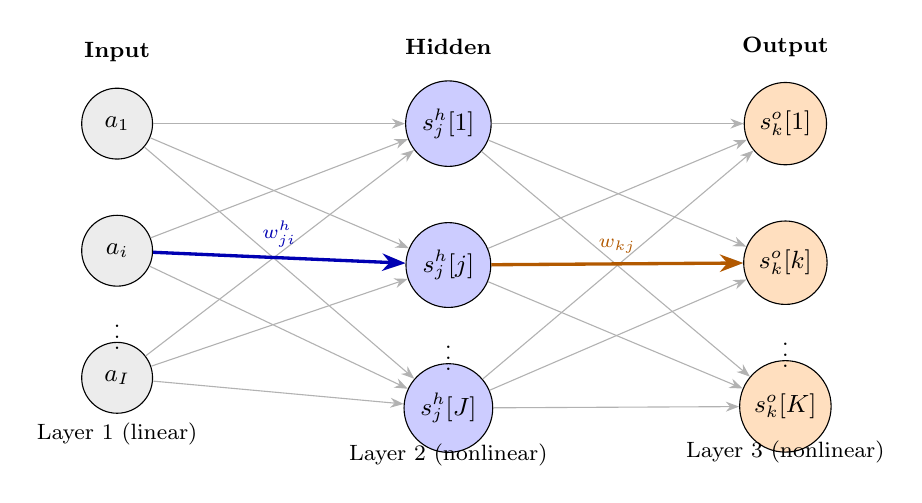
\begin{tikzpicture}[
    node distance=2.2cm and 3.0cm,
    neuron/.style={circle,draw,minimum size=0.9cm,font=\small},
    label/.style={font=\footnotesize},
    >=Stealth
  ]
  %% Input layer
  \node[neuron,fill=gray!15] (i1) {$a_1$};
  \node[neuron,fill=gray!15,below=0.7cm of i1] (i2) {$a_i$};
  \node[neuron,fill=gray!15,below=0.7cm of i2] (i3) {$a_I$};
  \node[label,above=0.2cm of i1] {\textbf{Input}};

  %% Hidden layer
  \node[neuron,fill=blue!20,right=3.2cm of i1] (h1) {$\sho[1]$};
  \node[neuron,fill=blue!20,below=0.7cm of h1] (h2) {$\sho[j]$};
  \node[neuron,fill=blue!20,below=0.7cm of h2] (h3) {$\sho[J]$};
  \node[label,above=0.2cm of h1] {\textbf{Hidden}};

  %% Output layer
  \node[neuron,fill=orange!25,right=3.2cm of h1] (o1) {$\sko[1]$};
  \node[neuron,fill=orange!25,below=0.7cm of o1] (o2) {$\sko[k]$};
  \node[neuron,fill=orange!25,below=0.7cm of o2] (o3) {$\sko[K]$};
  \node[label,above=0.2cm of o1] {\textbf{Output}};

  %% Dots
  \node[label,below=0.15cm of i2]  {$\vdots$};
  \node[label,below=0.15cm of h2]  {$\vdots$};
  \node[label,below=0.15cm of o2]  {$\vdots$};

  %% Input->Hidden edges
  \foreach \src in {i1,i2,i3}{
    \foreach \dst in {h1,h2,h3}{
      \draw[->,gray!60] (\src) -- (\dst);
    }
  }
  %% Label one weight
  \draw[->,very thick,blue!70!black] (i2) -- node[above,font=\scriptsize]{$\wji$} (h2);

  %% Hidden->Output edges
  \foreach \src in {h1,h2,h3}{
    \foreach \dst in {o1,o2,o3}{
      \draw[->,gray!60] (\src) -- (\dst);
    }
  }
  \draw[->,very thick,orange!70!black] (h2) -- node[above,font=\scriptsize]{$\wkj$} (o2);

  %% Layer labels on x-axis
  \node[label,below=1.6cm of i2]  {Layer 1 (linear)};
  \node[label,below=1.6cm of h2]  {Layer 2 (nonlinear)};
  \node[label,below=1.6cm of o2]  {Layer 3 (nonlinear)};
\end{tikzpicture}
\caption{Three-layer feed-forward neural network (Yegnanarayana Fig.\ 4.12
  reconstruction). Highlighted edges carry the weight notation used throughout
  the backpropagation derivation.}
\label{fig:three-layer}
\end{figure}

%% =============================================================================
\section{The Hard Learning Problem}
\label{sec:hard-learning}
%% =============================================================================

\subsection{Two Distinct Difficulties}

Students frequently conflate two different problems that arose in the history of
neural networks.  The instructors in this session took care to distinguish them
explicitly.

\begin{keyinsight}[title=Hard Problem vs.\ Hard Learning Problem]
\begin{description}[labelwidth=4.5cm,leftmargin=!]
  \item[Hard problem] A \emph{representation} difficulty: the data are not
        linearly separable, so a single-layer perceptron cannot solve the task
        (e.g.\ XOR).  Solved by adding hidden layers.
  \item[Hard learning problem] A \emph{training} difficulty: once hidden layers
        are added, we no longer have target outputs for hidden units, so we
        cannot compute the error signal needed to update the hidden-layer
        weights.
\end{description}
\end{keyinsight}

The hard learning problem caused the neural network field to stall for
roughly a decade until the backpropagation learning algorithm was
discovered/popularized in the 1980s.

\subsection{Why the Perceptron Rule Fails for Hidden Layers}

Recall \cref{eq:perceptron-rule}: the weight update requires the error
$(b_k - s_k)$.  For output-layer neurons we know the desired output $b_k$
directly from the training labels, so the error is computable.  For
hidden-layer neuron~$j$, however, we have \textbf{no} desired output --- the
``correct'' hidden-unit activation is not available in any dataset.  Hence
the perceptron rule cannot be applied to $\wji$.

\begin{remark}
\label{rem:why-hidden}
This is precisely why hidden layers are called \emph{hidden}: their targets are
hidden from us.  The backpropagation algorithm circumvents this by propagating
the \emph{output-layer error} backwards through the network to obtain a proxy
error signal for each hidden unit.
\end{remark}

\subsection{The Key Insight Behind Backpropagation}

Hidden unit~$j$ feeds into \emph{all} output neurons $k = 1,\ldots,K$.
Therefore it contributes a fraction of the total output error.  If we can
express the error at hidden unit~$j$ as a weighted sum of the output-layer
errors --- weighted by the connecting weights $\wkj$ --- we can update $\wji$
without needing explicit target outputs for the hidden layer.

\begin{keyinsight}[title=Core Backpropagation Idea]
Propagate the output error \emph{backward} through the network weights to
obtain a local error signal at every hidden unit, then use that signal to
update the preceding weights.  This requires that the activation function be
\emph{differentiable} everywhere.
\end{keyinsight}

\subsection{Why Differentiability is Non-Negotiable}

The step (signum) function used in the original perceptron has zero derivative
almost everywhere, which means no gradient information can flow backward through
it.  Replacing the step function with a smooth, differentiable nonlinearity
--- such as the sigmoid $\sigma(x) = 1/(1+e^{-x})$ or the
Rectified Linear Unit (ReLU) $f(x)=\max(0,x)$ --- gives a non-zero gradient
(almost everywhere) through which errors can be propagated.

\begin{equation}
  \text{Discrete (perceptron):}\quad
  \Delta w_i \propto (b - s)\cdot\text{sgn}'(\cdot) = 0
  \quad\Rightarrow\quad \text{no gradient.}
\end{equation}

\begin{equation}
  \text{Continuous (backprop):}\quad
  \Delta w_i \propto (b - s)\cdot f'(x)
  \quad\Rightarrow\quad \text{gradient available.}
  \label{eq:continuous-delta}
\end{equation}

The transition from the discrete to the continuous delta rule --- \cref{eq:continuous-delta}
--- is what the instructors call the move from the \emph{discrete perceptron
learning law} to the \emph{generalized delta rule}.

\begin{table}[htbp]
\centering
\caption{Comparison of single-layer and multi-layer learning rules.}
\label{tab:learning-rule-comparison}
\begin{tabularx}{\linewidth}{lXXX}
\toprule
\textbf{Property} & \textbf{Perceptron Rule} & \textbf{Delta Rule} & \textbf{Generalized Delta Rule (Backprop)} \\
\midrule
Activation $f$ & Signum (step) & Any differentiable & Any differentiable \\
Layers trained & Output only & Output only & All layers \\
Error signal & $b_k - s_k$ & $(b_k - s_k)\,f'(x_k)$ & Propagated from output \\
Requires $f'$ & No & Yes & Yes \\
Applicable to MLP & No & No & Yes \\
\bottomrule
\end{tabularx}
\end{table}

%% =============================================================================
\section{Backpropagation: Full Derivation}
\label{sec:backprop}
%% =============================================================================

We derive the backpropagation weight-update rules for both the output layer and
the hidden layer of the three-layer network in \cref{fig:three-layer}.

\subsection{Network Equations and Notation}

\paragraph{Hidden layer.}
\begin{align}
  \xho &= \sum_{i=1}^{I} \wji\,a_i + b_j^{h},
  \label{eq:hidden-net}\\
  \sho &= f(\xho).
  \label{eq:hidden-out}
\end{align}

\paragraph{Output layer.}
\begin{align}
  \xko &= \sum_{j=1}^{J} \wkj\,\sho + b_k^{o},
  \label{eq:output-net}\\
  \sko &= f(\xko).
  \label{eq:output-out}
\end{align}

\subsection{Total Error (Loss)}

For a single training pattern, the total squared error is

\begin{equation}
  E = \frac{1}{2}\sum_{k=1}^{K}\bigl(b_k - \sko\bigr)^{2},
  \label{eq:total-error}
\end{equation}

where the factor $\tfrac{1}{2}$ is included for notational convenience (it
cancels with the exponent when differentiated).

\begin{remark}
\label{rem:mse}
Averaged over all $P$ training patterns, \cref{eq:total-error} becomes the
Mean Squared Error (MSE):
\[
  \mathcal{L}_{\mathrm{MSE}}
  = \frac{1}{P}\sum_{p=1}^{P}\sum_{k=1}^{K}
    \bigl(b_k^{(p)} - s_k^{o(p)}\bigr)^{2}.
\]
\end{remark}

\subsection{Weight Update: Output Layer}
\label{sub:output-layer-update}

Applying gradient descent to \cref{eq:total-error} with respect to the
output-layer weight $\wkj$:

\begin{align}
  \Delta\wkj
  &= -\eta\,\pd{E}{\wkj}
  \label{eq:grad-desc}\\
  &= -\eta\,\pd{E}{\sko}\cdot\pd{\sko}{\xko}\cdot\pd{\xko}{\wkj}
  \tag{chain rule}\\
  &= -\eta\,\bigl[-(b_k - \sko)\bigr]\cdot f'(\xko)\cdot\sho
  \label{eq:output-intermediate}\\
  &= \eta\,(b_k - \sko)\,f'(\xko)\,\sho.
  \label{eq:output-update}
\end{align}

Define the \emph{output-layer error signal}:

\begin{equation}
  \deltak = (b_k - \sko)\,f'(\xko).
  \label{eq:delta-k}
\end{equation}

Then the update rule becomes

\begin{equation}
  \boxed{\Delta\wkj = \eta\,\deltak\,\sho.}
  \label{eq:output-rule-final}
\end{equation}

\subsection{Weight Update: Hidden Layer}
\label{sub:hidden-layer-update}

For the hidden-layer weight $\wji$:

\begin{align}
  \Delta\wji
  &= -\eta\,\pd{E}{\wji}\\
  &= -\eta\,\pd{E}{\sho}\cdot\pd{\sho}{\xho}\cdot\pd{\xho}{\wji}.
  \label{eq:hidden-chain}
\end{align}

The critical term is $\pd{E}{\sho}$.  Since $\sho$ feeds into every output
unit $k = 1,\ldots,K$ through $\xko = \sum_j \wkj\,\sho + b_k^{o}$, we
must sum over all output units:

\begin{align}
  \pd{E}{\sho}
  &= \sum_{k=1}^{K}\pd{E}{\sko}\cdot\pd{\sko}{\xko}\cdot\pd{\xko}{\sho}\\
  &= \sum_{k=1}^{K}\bigl[-(b_k - \sko)\bigr]\cdot f'(\xko)\cdot\wkj\\
  &= -\sum_{k=1}^{K}\deltak\,\wkj.
  \label{eq:error-prop-back}
\end{align}

\cref{eq:error-prop-back} is the \textbf{error back-propagation equation}: the
error at hidden unit~$j$ is a weighted sum of the output-layer error signals,
with weights equal to the forward connection weights $\wkj$.

Substituting back into \cref{eq:hidden-chain}:

\begin{align}
  \Delta\wji
  &= -\eta\cdot\Bigl(-\sum_{k=1}^{K}\deltak\,\wkj\Bigr)
     \cdot f'(\xho)\cdot a_i.
\end{align}

Define the \emph{hidden-layer error signal}:

\begin{equation}
  \deltajh = f'(\xho)\sum_{k=1}^{K}\deltak\,\wkj.
  \label{eq:delta-j-h}
\end{equation}

Then:

\begin{equation}
  \boxed{\Delta\wji = \eta\,\deltajh\,a_i.}
  \label{eq:hidden-rule-final}
\end{equation}

\subsection{General Weight Update Rule}

In both layers the update has the same form:

\begin{equation}
  w(m+1) = w(m) + \Delta w(m),
  \label{eq:general-update}
\end{equation}

or equivalently in gradient descent notation:

\begin{equation}
  \theta \leftarrow \theta - \eta\,\pd{\mathcal{L}}{\theta},
  \label{eq:gd-step}
\end{equation}

where $\theta$ is any trainable parameter (weight or bias).

\begin{keyinsight}[title=Structural Symmetry of Backpropagation]
Both update rules \cref{eq:output-rule-final,eq:hidden-rule-final} have the
form
\[
  \Delta w = \eta \times (\text{local error signal}) \times (\text{input to that weight}).
\]
This is the generalized delta rule.  The only difference between layers is how
the error signal is computed: output layer uses $(b_k - \sko)f'(\xko)$,
while hidden layer propagates errors backwards through $\sum_k \deltak\wkj$.
\end{keyinsight}

\subsection{Algorithm: Backpropagation Training}
\label{sub:backprop-algo}

\begin{algorithm}[H]
\caption{Backpropagation (Online / Stochastic)}
\label{alg:backprop}
\DontPrintSemicolon
\KwIn{Training set $\{(\mathbf{a}^{(p)},\mathbf{b}^{(p)})\}_{p=1}^{P}$;
       learning rate $\eta$; max epochs $M$}
\KwOut{Trained weights $\{\wji\}$, $\{\wkj\}$ and biases}
\BlankLine
Randomly initialise all weights and biases\;
\For{$m = 1$ \KwTo $M$}{
  \For{each pattern $p = 1$ \KwTo $P$}{
    \tcp{--- Forward Pass ---}
    Compute $\xho[j]$ via \cref{eq:hidden-net} for all $j$\;
    Compute $\sho[j] = f(\xho[j])$ for all $j$\;
    Compute $\xko[k]$ via \cref{eq:output-net} for all $k$\;
    Compute $\sko[k] = f(\xko[k])$ for all $k$\;
    Compute $E = \frac{1}{2}\sum_k(b_k^{(p)} - \sko[k])^2$\;
    \BlankLine
    \tcp{--- Backward Pass ---}
    \For{each output unit $k$}{
      $\deltak \leftarrow (b_k^{(p)} - \sko[k])\,f'(\xko[k])$\;
    }
    \For{each hidden unit $j$}{
      $\deltajh \leftarrow f'(\xho[j])\,\sum_{k=1}^{K}\deltak\,\wkj$\;
    }
    \BlankLine
    \tcp{--- Weight Update ---}
    \For{each output weight $\wkj$}{
      $\wkj \leftarrow \wkj + \eta\,\deltak\,\sho[j]$\;
    }
    \For{each hidden weight $\wji$}{
      $\wji \leftarrow \wji + \eta\,\deltajh\,a_i^{(p)}$\;
    }
  }
}
\end{algorithm}

%% =============================================================================
\section{Loss Computation and the Error Surface}
\label{sec:loss}
%% =============================================================================

\subsection{Mean Squared Error (MSE)}
\label{sub:mse}

For a regression task, the standard loss function is the Mean Squared Error.
For a single training example with true label $y$ and network prediction
$\hat{y}$:

\begin{equation}
  \mathcal{L} = (y - \hat{y})^{2}.
  \label{eq:se}
\end{equation}

Averaged over $N$ data points:

\begin{equation}
  \mathcal{L}_{\mathrm{MSE}}
  = \frac{1}{N}\sum_{i=1}^{N}(y_i - \hat{y}_i)^{2}.
  \label{eq:mse}
\end{equation}

\begin{example}[title=Numerical MSE Computation (Slide V03)]
Consider the toy IQ/CGPA $\to$ LPA network from the lecture.  For the first
training example the network outputs $\hat{y} = 10.36$ against the true label
$y = 3$:
\[
  \mathcal{L} = (3 - 10.36)^{2} = (-7.36)^{2} = 54.17.
\]
After one iteration of backpropagation the updated weights yield
$\hat{y} = 0.99$, giving:
\[
  \mathcal{L}_{\mathrm{new}} = (3 - 0.99)^{2} = (2.01)^{2} \approx 4.04.
\]
A dramatic reduction in loss from a \emph{single} gradient step illustrates
the efficiency of backpropagation when the learning rate is appropriately
chosen.
\end{example}

\subsection{Properties of MSE}

\begin{table}[htbp]
\centering
\caption{Properties of common loss functions for neural network training.}
\label{tab:loss-comparison}
\begin{tabularx}{\linewidth}{lXXX}
\toprule
\textbf{Property} & \textbf{MSE} & \textbf{MAE} & \textbf{Cross-Entropy} \\
\midrule
Non-negative & Yes & Yes & Yes \\
Zero at perfect prediction & Yes & Yes & Yes \\
Differentiable everywhere & Yes & No (at 0) & Yes \\
Penalises large errors & Quadratic & Linear & --- \\
Typical task & Regression & Regression & Classification \\
\bottomrule
\end{tabularx}
\end{table}

The differentiability of MSE is essential: the gradient of the loss with
respect to the network output is

\begin{equation}
  \pd{\mathcal{L}}{\hat{y}} = 2(\hat{y} - y),
  \label{eq:mse-grad}
\end{equation}

which is linear in the prediction error and therefore always provides a useful
training signal.

\subsection{Gradient of the Loss: Chain Rule Through the Network}
\label{sub:chain-rule}

For the toy network (IQ, CGPA $\to h_1, h_2 \to \hat{y}$) from the slides:

\begin{align}
  Z_1 &= W_{11}X_1 + W_{12}X_2 + B_1,\\
  H_1 &= \text{ReLU}(Z_1),\\
  Z_2 &= W_{21}X_1 + W_{22}X_2 + B_2,\\
  H_2 &= \text{ReLU}(Z_2),\\
  \hat{y} &= V_1 H_1 + V_2 H_2 + B_3,\\
  \mathcal{L} &= (Y - \hat{y})^{2}.
\end{align}

The partial derivatives required by backpropagation are:

\begin{align}
  \pd{\mathcal{L}}{\hat{y}} &= 2(\hat{y} - Y),
  \label{eq:dl-dyhat}\\
  \pd{\mathcal{L}}{V_1} &= \pd{\mathcal{L}}{\hat{y}}\cdot H_1
    = 2(\hat{y}-Y)\,H_1,\\
  \pd{\mathcal{L}}{V_2} &= 2(\hat{y}-Y)\,H_2,\\
  \pd{\mathcal{L}}{B_3} &= 2(\hat{y}-Y),\\
  \pd{\mathcal{L}}{W_{11}} &=
    \pd{\mathcal{L}}{\hat{y}}\cdot\pd{\hat{y}}{H_1}
    \cdot\pd{H_1}{Z_1}\cdot\pd{Z_1}{W_{11}}
    = 2(\hat{y}-Y)\cdot V_1\cdot\text{ReLU}'(Z_1)\cdot X_1,
  \label{eq:dl-dw11}\\
  \pd{\mathcal{L}}{W_{12}} &= 2(\hat{y}-Y)\cdot V_1\cdot\text{ReLU}'(Z_1)\cdot X_2.
\end{align}

The ReLU derivative is:

\begin{equation}
  \text{ReLU}'(z) =
  \begin{cases}
    1 & \text{if } z > 0,\\
    0 & \text{if } z \leq 0.
  \end{cases}
  \label{eq:relu-deriv}
\end{equation}

\subsection{The Error Surface: Convex vs.\ Non-Convex}
\label{sub:error-surface}

At timestamp 00:48:20 of the lecture video the instructor displayed search
results for ``loss function convex curve'' to motivate the discussion of
optimization challenges.

\begin{figure}[htbp]
\centering
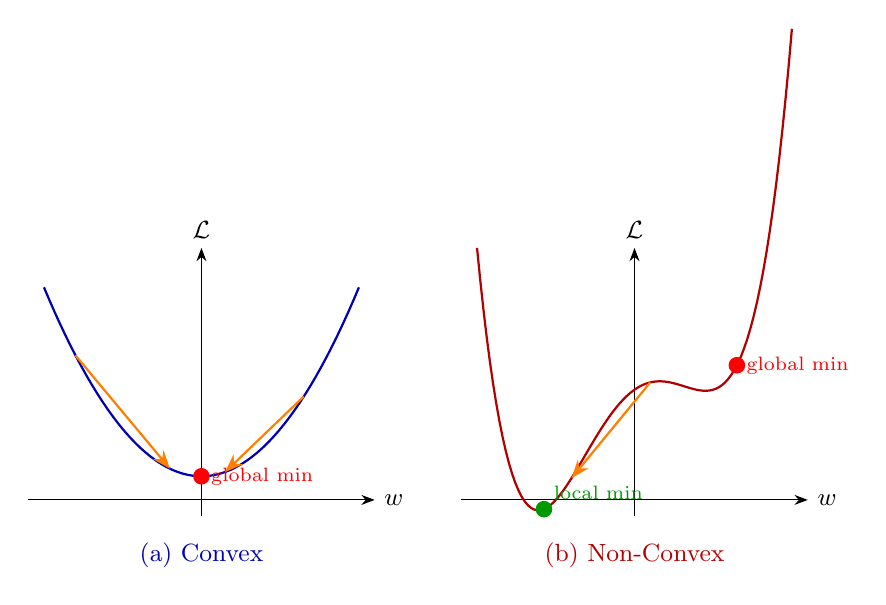
\begin{tikzpicture}[>=Stealth, scale=1.0]
  %% Left: Convex
  \begin{scope}[xshift=0cm]
    \draw[->] (-2.2,0) -- (2.2,0) node[right,font=\small]{$w$};
    \draw[->] (0,-0.2) -- (0,3.2) node[above,font=\small]{$\mathcal{L}$};
    \draw[thick,blue!70!black,domain=-2:2,samples=60]
      plot (\x, {0.6*\x*\x + 0.3});
    \fill[red] (0,0.3) circle (3pt) node[right,font=\scriptsize]{global min};
    \draw[->,orange,thick] (-1.6,{0.6*1.6*1.6+0.3}) -- (-0.4,{0.6*0.4*0.4+0.3});
    \draw[->,orange,thick] (1.3,{0.6*1.3*1.3+0.3}) -- (0.3,{0.6*0.3*0.3+0.3});
    \node[font=\small,blue!70!black] at (0,-0.7) {(a) Convex};
  \end{scope}
  %% Right: Non-convex
  \begin{scope}[xshift=5.5cm]
    \draw[->] (-2.2,0) -- (2.2,0) node[right,font=\small]{$w$};
    \draw[->] (0,-0.2) -- (0,3.2) node[above,font=\small]{$\mathcal{L}$};
    \draw[thick,red!70!black,domain=-2:2,samples=100]
      plot (\x, {0.5*\x*\x*\x*\x - 1.2*\x*\x + 0.7*\x + 1.4});
    \fill[green!60!black] (-1.15,{0.5*1.15^4 - 1.2*1.15^2 - 0.7*1.15 + 1.4}) circle (3pt)
      node[above right,font=\scriptsize]{local min};
    \fill[red] (1.3,{0.5*1.3^4 - 1.2*1.3^2 + 0.7*1.3 + 1.4}) circle (3pt)
      node[right,font=\scriptsize]{global min};
    \draw[->,orange,thick] (0.2,{0.5*0.2^4-1.2*0.2^2+0.7*0.2+1.4})
      -- (-0.8,{0.5*0.8^4-1.2*0.8^2-0.7*0.8+1.4});
    \node[font=\small,red!70!black] at (0,-0.7) {(b) Non-Convex};
  \end{scope}
\end{tikzpicture}
\caption{Schematic loss surfaces: (a) convex --- gradient descent always
  converges to the unique global minimum; (b) non-convex --- gradient descent
  may get trapped in a local minimum.  Neural network loss surfaces are
  generally non-convex.}
\label{fig:loss-surface}
\end{figure}

\begin{keyinsight}[title=Convex vs.\ Non-Convex Implications]
\begin{itemize}[noitemsep]
  \item A \textbf{convex} loss surface has a single global minimum.  Gradient
        descent with any positive learning rate is guaranteed to converge.
  \item A \textbf{non-convex} loss surface has multiple local minima and saddle
        points.  Standard gradient descent may get stuck.
  \item Neural network loss surfaces are \textbf{generally non-convex}.  This
        motivates advanced optimizers (SGD with momentum, Adam, RMSProp) and
        careful weight initialisation strategies.
\end{itemize}
\end{keyinsight}

\subsection{Effect of the Learning Rate on Gradient Descent}

The learning rate $\eta$ controls the step size along the negative gradient
direction.  From the discussion in the session:

\begin{itemize}[noitemsep]
  \item If $\eta$ is \textbf{too large}: the update step overshoots the
        minimum, potentially causing the loss to \emph{increase} or oscillate.
  \item If $\eta$ is \textbf{too small}: convergence is very slow, and
        training may take impractically many epochs.
  \item \textbf{Gradient magnitude matters}: when gradients are very large
        (e.g.\ $\approx 97$ in the numerical example), a small $\eta$ such as
        $10^{-4}$ is necessary to keep the step size reasonable.
\end{itemize}

\begin{warningbox}[title=Exploding and Vanishing Gradients]
Two pathological regimes arise during backpropagation in deep networks:
\begin{description}[noitemsep]
  \item[Exploding gradients:] Gradients grow exponentially with depth.
        Observed in the session when $\partial\mathcal{L}/\partial V_1 \approx 97$,
        $\partial\mathcal{L}/\partial W_{11} \approx 1413$.
        Remedy: gradient clipping, careful initialisation, batch normalisation.
  \item[Vanishing gradients:] Gradients shrink exponentially with depth,
        halting learning in early layers.
        Remedy: ReLU activation (avoids sigmoid saturation), residual connections,
        careful initialisation (Xavier, He).
\end{description}
The instructor noted that these topics would be covered in the following session.
\end{warningbox}

%% =============================================================================
\section{Numerical Walk-Through: Toy IQ/CGPA Network}
\label{sec:numerical}
%% =============================================================================

\subsection{Network Architecture}

The toy dataset used throughout the session predicts salary (LPA) from IQ and
CGPA:

\begin{center}
\begin{tabular}{ccc}
\toprule
IQ ($X_1$) & CGPA ($X_2$) & LPA ($Y$) \\
\midrule
80 & 8  & 3 \\
60 & 9  & 4 \\
75 & 7  & 8 \\
127 & ?  & 11 \\
\bottomrule
\end{tabular}
\end{center}

The network has 2 input neurons, 2 hidden neurons (ReLU), and 1 output neuron
(linear).  Initial weights:

\begin{align*}
  W_{11} = 0.02,\quad W_{12} = 0.50,\quad
  W_{21} = 0.04,\quad W_{22} = -0.30,\\
  V_1 = 1.20,\quad V_2 = 0.80,\quad
  B_1 = B_2 = B_3 = 1.0.
\end{align*}

\subsection{Forward Pass (Pattern 1: $X_1=80$, $X_2=8$, $Y=3$)}

\begin{align}
  Z_1 &= 0.02\times80 + 0.50\times8 + 1 = 1.6 + 4.0 + 1 = 6.6,\\
  H_1 &= \text{ReLU}(6.6) = 6.6,\\
  Z_2 &= 0.04\times80 + (-0.30)\times8 + 1 = 3.2 - 2.4 + 1 = 1.8,\\
  H_2 &= \text{ReLU}(1.8) = 1.8,\\
  \hat{y} &= 1.20\times6.6 + 0.80\times1.8 + 1.0 = 7.92 + 1.44 + 1.0 = 10.36,\\
  \mathcal{L} &= (3 - 10.36)^{2} = 54.17.
\end{align}

\subsection{Backward Pass (Selected Gradients)}

\begin{align}
  \pd{\mathcal{L}}{\hat{y}} &= 2(10.36 - 3) = 14.72,\\
  \pd{\mathcal{L}}{V_1} &= 14.72\times 6.6 = 97.15,\\
  \pd{\mathcal{L}}{V_2} &= 14.72\times 1.8 = 26.50,\\
  \pd{\mathcal{L}}{B_3} &= 14.72,\\
  \pd{\mathcal{L}}{W_{11}} &= 14.72\times1.2\times1.0\times80 = 1412.9.
\end{align}

The large gradient values (97, 26, 1413) motivate the choice of
$\eta = 10^{-4}$.

\subsection{Weight Update and Iteration 2}

\begin{align}
  V_1^{\mathrm{new}} &= 1.20 - 10^{-4}\times97.15 \approx 1.190,\\
  V_2^{\mathrm{new}} &= 0.80 - 10^{-4}\times26.50 \approx 0.797,\\
  B_3^{\mathrm{new}} &= 1.00 - 10^{-4}\times14.72 \approx 0.9985,\\
  W_{11}^{\mathrm{new}} &= 0.02 - 10^{-4}\times1412.9 \approx -0.121.
\end{align}

After updating all nine parameters and repeating the forward pass:

\begin{equation}
  \hat{y}^{(2)} \approx 0.99,\qquad
  \mathcal{L}^{(2)} = (3 - 0.99)^{2} \approx 4.04.
\end{equation}

A reduction from 54.17 to 4.04 --- a factor of $\approx\!13\times$ improvement
--- in \emph{one} gradient step.

\begin{example}[title=Interpreting Weight Direction Change]
A student asked why all weights decreased in iteration~1.  The instructor
explained with reference to the loss surface: the sign of the weight update
depends on which side of the minimum the current weight value lies.
\begin{itemize}[noitemsep]
  \item If we are on the \emph{right} side of the minimum (positive gradient),
        the weight decreases.
  \item If we are on the \emph{left} side (negative gradient), the weight
        increases.
\end{itemize}
Since only one iteration was shown, and the initialisation happened to place
all parameters on the right side, all weights decreased.  In general both
directions are possible.
\end{example}

%% =============================================================================
\section{PyTorch Implementation}
\label{sec:pytorch}
%% =============================================================================

\subsection{Version 1: Manual Backpropagation}
\label{sub:manual-backprop}

The instructor implemented the complete forward and backward passes from
scratch in PyTorch, using only scalar tensor arithmetic (no \texttt{nn.Module},
no built-in loss, no optimizer).

\subsubsection{Data and Weight Initialisation}

\begin{verbatim}
import torch

# Dataset tensors
X = torch.tensor([[80., 8.], [60., 9.], [75., 7.], [127., 12.]])
Y = torch.tensor([[3.], [4.], [8.], [11.]])

# Weight initialisation (matching the numerical example)
W11 = torch.tensor(0.02); W12 = torch.tensor(0.50)
W21 = torch.tensor(0.04); W22 = torch.tensor(-0.30)
V1  = torch.tensor(1.20); V2  = torch.tensor(0.80)
B1  = torch.tensor(1.0);  B2  = torch.tensor(1.0);  B3 = torch.tensor(1.0)

lr     = 1e-4
epochs = 2
loss_history = []
\end{verbatim}

\subsubsection{Activation Functions (Defined from Scratch)}

\begin{verbatim}
def relu(x):
    return torch.where(x > 0, x, torch.tensor(0.0))

def relu_derivative(x):
    return torch.where(x > 0, torch.tensor(1.0), torch.tensor(0.0))
\end{verbatim}

\subsubsection{Training Loop (One Row at a Time)}

\begin{verbatim}
for epoch in range(epochs):
    total_loss = 0.0
    for i in range(len(X)):
        X1, X2 = X[i, 0], X[i, 1]
        target  = Y[i, 0]

        # ─── Forward pass ───────────────────────────────────────────
        Z1   = W11*X1 + W12*X2 + B1
        H1   = relu(Z1)
        Z2   = W21*X1 + W22*X2 + B2
        H2   = relu(Z2)
        yhat = V1*H1 + V2*H2 + B3
        loss = (target - yhat)**2
        total_loss += loss

        # ─── Backward pass ──────────────────────────────────────────
        DL_Dyhat = 2*(yhat - target)
        DV1  = DL_Dyhat * H1
        DV2  = DL_Dyhat * H2
        DB3  = DL_Dyhat

        DL_DH1 = DL_Dyhat * V1
        DH1_DZ1 = relu_derivative(Z1)
        DW11 = DL_DH1 * DH1_DZ1 * X1
        DW12 = DL_DH1 * DH1_DZ1 * X2
        DB1  = DL_DH1 * DH1_DZ1

        DL_DH2 = DL_Dyhat * V2
        DH2_DZ2 = relu_derivative(Z2)
        DW21 = DL_DH2 * DH2_DZ2 * X1
        DW22 = DL_DH2 * DH2_DZ2 * X2
        DB2  = DL_DH2 * DH2_DZ2

        # ─── Parameter update ────────────────────────────────────────
        W11 -= lr * DW11;  W12 -= lr * DW12
        W21 -= lr * DW21;  W22 -= lr * DW22
        V1  -= lr * DV1;   V2  -= lr * DV2
        B1  -= lr * DB1;   B2  -= lr * DB2;  B3 -= lr * DB3

    loss_history.append(total_loss.item())
    print(f"Epoch {epoch+1}: loss = {total_loss.item():.4f}")
\end{verbatim}

\subsection{Version 2: PyTorch Autograd}
\label{sub:autograd}

In the second version the instructor introduced \texttt{torch.autograd},
PyTorch's automatic differentiation engine.  By setting
\texttt{requires\_grad=True} on each parameter tensor, PyTorch automatically
builds a computation graph during the forward pass and computes all gradients
via a single call to \texttt{loss.backward()}.

\begin{verbatim}
# Weights with gradient tracking
W11 = torch.tensor(0.02, requires_grad=True)
W12 = torch.tensor(0.50, requires_grad=True)
# ... (same for all parameters) ...

# Inside training loop:
yhat = V1*H1 + V2*H2 + B3
loss = (target - yhat)**2

loss.backward()   # Autograd computes ALL gradients

with torch.no_grad():
    W11 -= lr * W11.grad
    # ... update all parameters ...

# Zero gradients before next iteration
W11.grad.zero_()
# ... zero all grads ...
\end{verbatim}

\begin{keyinsight}[title=Manual vs.\ Autograd Verification]
A key pedagogical goal of the session was to show that the gradients computed
manually match those computed by Autograd to numerical precision.  This
verification confirms that the chain-rule derivation in
\cref{sec:backprop} is correct and builds trust in the Autograd abstraction
before using it blindly in future sessions.
\end{keyinsight}

\subsection{Weight Initialisation Strategies}
\label{sub:weight-init}

A student asked whether the initial weight values affect convergence.  The
instructor confirmed that they do and previewed the following techniques
(to be covered in depth in later sessions):

\begin{table}[htbp]
\centering
\caption{Common weight initialisation strategies.}
\label{tab:weight-init}
\begin{tabularx}{\linewidth}{lXX}
\toprule
\textbf{Method} & \textbf{Distribution} & \textbf{Best for} \\
\midrule
Zero init & $w = 0$ & Not recommended (symmetry breaking failure) \\
Random uniform & $w \sim \mathcal{U}(-1,1)$ & Simple, but may cause vanishing/exploding gradients \\
Xavier (Glorot) & $w \sim \mathcal{U}\!\left(-\sqrt{6/(n_\text{in}+n_\text{out})},\sqrt{6/(n_\text{in}+n_\text{out})}\right)$ & Sigmoid/Tanh activations \\
He (Kaiming) & $w \sim \mathcal{N}(0, 2/n_\text{in})$ & ReLU activations \\
\bottomrule
\end{tabularx}
\end{table}

%% =============================================================================
\section{Activation Functions: From Step to Differentiable}
\label{sec:activations}
%% =============================================================================

\subsection{The Sigmoid Function}

The logistic sigmoid was historically the first differentiable nonlinearity
used to replace the perceptron step function:

\begin{equation}
  \sigma(x) = \frac{1}{1 + e^{-x}},\qquad
  \sigma'(x) = \sigma(x)\bigl(1 - \sigma(x)\bigr).
  \label{eq:sigmoid}
\end{equation}

The derivative $\sigma'(x)$ is non-zero for all $x \in \mathbb{R}$, which
enables error propagation.  However, for $|x| \gg 1$ the derivative is
very close to zero (saturation), leading to the \emph{vanishing gradient}
problem in deep networks.

\subsection{The Rectified Linear Unit (ReLU)}

\begin{equation}
  \text{ReLU}(x) = \max(0, x) =
  \begin{cases} x & x > 0,\\ 0 & x \leq 0. \end{cases}
  \label{eq:relu}
\end{equation}

ReLU has become the default activation in modern deep learning because:
\begin{enumerate}[noitemsep]
  \item Its derivative is 1 for all positive inputs (no gradient saturation on
        the positive side).
  \item It is computationally cheap.
  \item It empirically works better than sigmoid in most deep architectures.
\end{enumerate}

The instructor stressed that \emph{any} differentiable nonlinear function can
be used --- the choice is guided by empirical performance and specific task
requirements.

\subsection{Comparison of Activation Functions}

\begin{table}[htbp]
\centering
\caption{Properties of activation functions discussed in the session.}
\label{tab:activations}
\begin{tabularx}{\linewidth}{lXXXX}
\toprule
\textbf{Function} & \textbf{Range} & \textbf{Differentiable} & \textbf{Vanishing Grad?} & \textbf{Common Use} \\
\midrule
Signum (step) & $\{-1,+1\}$ & No (at 0) & N/A & Perceptron \\
Sigmoid & $(0,1)$ & Yes & Yes (deep nets) & Binary output \\
Tanh & $(-1,1)$ & Yes & Yes (deep nets) & RNN gates \\
ReLU & $[0,\infty)$ & No (at 0) & No (positive side) & Hidden layers \\
Leaky ReLU & $(-\infty,\infty)$ & Yes & No & Hidden layers \\
\bottomrule
\end{tabularx}
\end{table}

%% =============================================================================
\section{Summary and Conclusion}
\label{sec:summary}
%% =============================================================================

\subsection{Key Concepts Covered}

Session~06 completed the theoretical backbone of feedforward ANNs.  The
following core ideas were developed:

\begin{enumerate}[label=\arabic*.,noitemsep]
  \item \textbf{Hard problem vs.\ hard learning problem.}  The hard problem
        (linear inseparability) is solved by adding hidden layers.  The hard
        learning problem (no target outputs for hidden units) is solved by
        backpropagation.

  \item \textbf{Role of differentiability.}  Replacing the step function with
        a differentiable activation (sigmoid, ReLU) is the critical enabler of
        backpropagation.  Without a non-zero derivative, the error signal
        cannot be propagated backward.

  \item \textbf{Generalized delta rule.}  Backpropagation is a direct
        generalization of the single-layer delta rule.  The update formula
        $\Delta w = \eta \cdot \delta \cdot \text{input}$ holds at every layer,
        with $\delta$ computed via the chain rule.

  \item \textbf{MSE loss.}  The squared error $(y - \hat{y})^2$ and its mean
        over the dataset provide a differentiable training objective whose
        gradient is $2(\hat{y}-y)$.

  \item \textbf{Convex vs.\ non-convex surfaces.}  Neural network loss
        landscapes are non-convex.  Gradient descent behavior (weight
        increase or decrease) depends on which side of a minimum the current
        parameters lie.

  \item \textbf{Learning rate selection.}  A learning rate of $\eta = 10^{-4}$
        was necessary because the raw gradients were of order $10^2$--$10^3$.
        Poor learning rate choice leads to exploding gradients (too large) or
        extremely slow convergence (too small).

  \item \textbf{PyTorch Autograd.}  The automatic differentiation system
        eliminates the need to hand-code gradients.  Its results match manual
        derivations exactly, confirming correctness of the theory.
\end{enumerate}

\subsection{Formulae Reference Card}

\begin{keyinsight}[title=Essential Backpropagation Formulae]
\begin{align*}
  &\textbf{Output layer error signal:}
  &\deltak &= (b_k - \sko)\,f'(\xko)\\
  &\textbf{Output layer weight update:}
  &\Delta\wkj &= \eta\,\deltak\,\sho\\
  &\textbf{Hidden layer error signal:}
  &\deltajh &= f'(\xho)\sum_{k=1}^{K}\deltak\,\wkj\\
  &\textbf{Hidden layer weight update:}
  &\Delta\wji &= \eta\,\deltajh\,a_i\\
  &\textbf{General update:}
  &\theta &\leftarrow \theta - \eta\,\pd{\mathcal{L}}{\theta}
\end{align*}
\end{keyinsight}

\subsection{Looking Ahead}

The next session will continue from this foundation by examining:

\begin{itemize}[noitemsep]
  \item Vanishing and exploding gradient problems in depth.
  \item Weight initialisation techniques (Xavier, He).
  \item Batch normalisation and its role in stabilising training.
  \item Advanced optimizers beyond plain SGD.
\end{itemize}

The instructor's advice to students: practice the PyTorch Colab notebook
independently, vary the learning rate and initial weights, and observe the
effect on loss convergence.  A firm grasp of this two-layer example is the
foundation for understanding any deeper architecture.

\vspace{1cm}
\hrule
\vspace{0.4cm}
{\small
\textbf{Source materials:}
Transcript: \texttt{session06\_transcript.vtt};
Visual extraction: \texttt{session06\_visual\_extraction.md};
Slide deck: \texttt{02-DL-NNIntro} (slides 50--87/87).
Reference: B.\ Yegnanarayana, \textit{Artificial Neural Networks}, PHI,
New Delhi, 1999.
}

\clearpage

%% ============================================================
%% Session 07: Backpropagation Worked Example and Gradient Descent
%% ============================================================
\part{Session 07: Backpropagation Worked Example and Gradient Descent}

%% ── Title page ───────────────────────────────────────────────────────────────
\begin{titlepage}
  \centering
  \vspace*{2cm}
  {\LARGE\bfseries Deep Learning: Advanced ANN Concepts\par}
  \vspace{0.5cm}
  {\large Lecture Notes -- Session 07\par}
  \vspace{1.5cm}
  \rule{\linewidth}{0.5pt}\\[0.4cm]
  {\huge\bfseries Backpropagation Worked Example\\[0.3cm]
   \& Gradient Descent\par}
  \rule{\linewidth}{0.5pt}\\[1.5cm]

  \begin{tabular}{ll}
    \textbf{Session}     & 07 \\[4pt]
    \textbf{Topic}       & Backpropagation numerical example; chain-rule derivation \\
                         & for all 9 parameters; learning rate; gradient descent \\[4pt]
    \textbf{Deck}        & \texttt{03-DL-ANNAdvancedConcepts} \\[4pt]
    \textbf{Instructors} & Prof.\ S R M Prasanna \& Dr.\ Sunil Saumya \\[4pt]
    \textbf{Institute}   & IIIT Dharwad \\[4pt]
    \textbf{Duration}    & $\approx 1$h $39$m \\[4pt]
    \textbf{Video}       & \url{https://vimeo.com/1144571367} \\
  \end{tabular}

  \vfill
  {\large\itshape Course: Deep Learning -- Advanced ANN Concepts\par}
\end{titlepage}

%% ── Table of Contents ────────────────────────────────────────────────────────

\newpage

% =============================================================================
\section{Introduction}
\label{sec:intro}
% =============================================================================

Session~07 sits at the boundary between \emph{first-level} and
\emph{advanced-level} understanding of artificial neural networks.
The first six sessions established the perceptron, multi-layer perceptrons,
forward propagation, and the conceptual role of backpropagation.
This session consolidates that foundation by working through every arithmetic
step of a complete backpropagation pass, then transitions to the key concepts
needed to train networks reliably in practice:

\begin{itemize}[leftmargin=2em]
  \item A full numerical forward pass on a 2-input, 2-hidden-neuron,
        1-output network (IQ/CGPA $\to$ placement-salary prediction).
  \item Exact computation of all 9 gradients via the chain rule.
  \item One complete parameter update with learning rate $\eta = 10^{-4}$,
        demonstrating a 92.6\% drop in loss ($54.17 \to 4.006$) in a single
        step.
  \item Intuition behind gradient descent and why the update rule
        $\theta \leftarrow \theta - \eta\,\pderiv{\Loss}{\theta}$ always
        moves toward the minimum.
  \item Three variants of gradient descent --- batch, stochastic, and
        mini-batch --- with trade-off analysis.
  \item PyTorch implementation hints for each variant.
\end{itemize}

The material applies directly to every deeper architecture (CNN, RNN, LSTM)
studied in later sessions: the chain-rule mechanics, the update rule, and the
gradient-descent variants are universal.

% =============================================================================
\section{Background and Prerequisites}
\label{sec:background}
% =============================================================================

\subsection{The Network Architecture}

Throughout this session the instructors use a fixed toy network:
two inputs $x_1, x_2$, two hidden neurons producing activations $h_1, h_2$,
and one linear output neuron $\yhat$.
The task is regression: predict a numeric placement salary (LPA) from
IQ score and CGPA.

\begin{definition}[Feedforward Neural Network -- Session Notation]
\label{def:ffnn}
A \emph{feedforward neural network} with one hidden layer computes:
\begin{align}
  z_k &= \sum_j w_{kj}\,x_j + b_k, \qquad k=1,2 \label{eq:hidden-preact}\\
  h_k &= \ReLU(z_k) = \max(0,\, z_k), \qquad k=1,2 \label{eq:relu}\\
  \yhat &= v_1 h_1 + v_2 h_2 + b_3. \label{eq:output}
\end{align}
The squared-error loss for one sample $(x_1,x_2,y)$ is
\begin{equation}
  \Loss = (\yhat - y)^2. \label{eq:loss}
\end{equation}
\end{definition}

\subsection{Parameter Inventory}

The 9 trainable parameters are:
\[
  \Theta = \{w_{11},\, w_{12},\, w_{21},\, w_{22},\, b_1,\, b_2,\, v_1,\, v_2,\, b_3\}.
\]

\subsection{The ReLU Activation and Its Derivative}

\begin{definition}[ReLU]
\label{def:relu}
$\ReLU(z) = \max(0,z)$, with sub-gradient
\begin{equation}
  \frac{d\,\ReLU}{dz}(z) = \mathbf{1}[z > 0] =
  \begin{cases} 1 & z > 0 \\ 0 & z \leq 0. \end{cases}
  \label{eq:relu-deriv}
\end{equation}
\end{definition}

\begin{keyinsight}
ReLU's derivative is either 0 or 1 --- never a tiny fraction.
This prevents the \emph{vanishing gradient problem} that plagued
sigmoid-based networks, and is the main reason ReLU became the
default hidden-layer activation.
\end{keyinsight}

\subsection{Chain Rule (Univariate)}

For a composed function $\Loss = f(g(\theta))$:
\begin{equation}
  \pderiv{\Loss}{\theta} = \pderiv{\Loss}{g} \cdot \pderiv{g}{\theta}.
  \label{eq:chain-rule}
\end{equation}
Backpropagation applies \cref{eq:chain-rule} recursively, propagating
partial derivatives from the output layer back through each hidden layer.

% =============================================================================
\section{Forward Pass: Numerical Worked Example}
\label{sec:forward}
% =============================================================================

\subsection{Initial Parameter Values}

The session begins with the following hand-crafted initial values
(first row of the toy dataset):

\begin{center}
\begin{tabular}{lll}
\toprule
\textbf{Quantity} & \textbf{Symbol} & \textbf{Value} \\
\midrule
Input 1 (IQ)    & $x_1$ & $80$ \\
Input 2 (CGPA)  & $x_2$ & $8$  \\
Target (LPA)    & $y$   & $3$  \\
\midrule
Hidden weight   & $w_{11}$ & $0.02$ \\
Hidden weight   & $w_{12}$ & $0.50$ \\
Hidden weight   & $w_{21}$ & $0.04$ \\
Hidden weight   & $w_{22}$ & $-0.30$ \\
Hidden bias     & $b_1$    & $1$ \\
Hidden bias     & $b_2$    & $1$ \\
Output weight   & $v_1$    & $1.2$ \\
Output weight   & $v_2$    & $0.8$ \\
Output bias     & $b_3$    & $1$ \\
\bottomrule
\end{tabular}
\end{center}

\subsection{Step-by-Step Computation}

\paragraph{Hidden neuron 1.}
\begin{align}
  z_1 &= w_{11} x_1 + w_{12} x_2 + b_1
       = 0.02\cdot80 + 0.5\cdot8 + 1
       = 1.6 + 4.0 + 1.0 = 6.6, \label{eq:z1}\\
  h_1 &= \ReLU(6.6) = 6.6. \label{eq:h1}
\end{align}

\paragraph{Hidden neuron 2.}
\begin{align}
  z_2 &= w_{21} x_1 + w_{22} x_2 + b_2
       = 0.04\cdot80 + (-0.3)\cdot8 + 1
       = 3.2 - 2.4 + 1.0 = 1.8, \label{eq:z2}\\
  h_2 &= \ReLU(1.8) = 1.8. \label{eq:h2}
\end{align}

\paragraph{Output neuron.}
\begin{align}
  \yhat &= v_1 h_1 + v_2 h_2 + b_3
         = 1.2\cdot6.6 + 0.8\cdot1.8 + 1
         = 7.92 + 1.44 + 1.0 = 10.36. \label{eq:yhat}
\end{align}

\paragraph{Loss.}
\begin{equation}
  \Loss = (\yhat - y)^2 = (10.36 - 3)^2 = (7.36)^2 \approx 54.17.
  \label{eq:loss-val}
\end{equation}

\begin{example}[Why is the initial prediction so poor?]
$x_1 = 80$ is a large number.
With $w_{11} = 0.02$, the pre-activation $z_1 = 6.6$ is already large,
and after multiplying by $v_1 = 1.2$ the network predicts $\yhat = 10.36$
when the target is only $y = 3$.
This illustrates why \emph{input normalisation} is important in practice:
unscaled features cause large pre-activations and correspondingly large
gradients, which destabilise training.
\end{example}

\subsection{Network Diagram}

\cref{fig:network} shows the architecture with the numerical values annotated
on each connection.

\begin{figure}[ht]
\centering
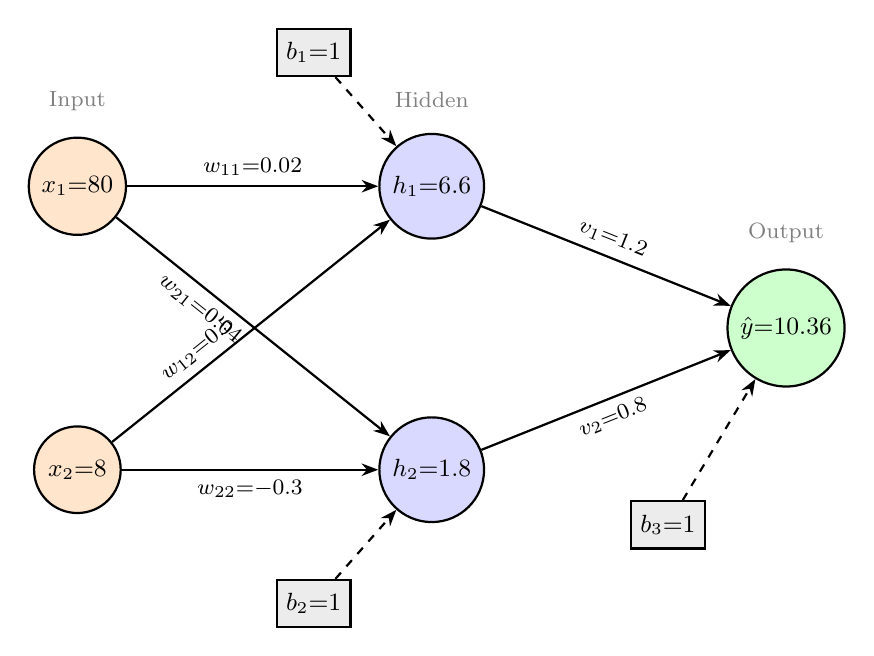
\begin{tikzpicture}[
    neuron/.style={circle,draw,minimum size=1.1cm,thick},
    bias/.style={rectangle,draw,minimum size=0.6cm,fill=gray!15,thick},
    arr/.style={-{Stealth[length=6pt]},thick},
    font=\small
  ]
  %% Input layer
  \node[neuron,fill=orange!20] (x1) at (0, 1.8) {$x_1{=}80$};
  \node[neuron,fill=orange!20] (x2) at (0,-1.8) {$x_2{=}8$};

  %% Hidden layer
  \node[neuron,fill=blue!15]  (h1) at (4.5, 1.8) {$h_1{=}6.6$};
  \node[neuron,fill=blue!15]  (h2) at (4.5,-1.8) {$h_2{=}1.8$};
  \node[bias] (b1) at (3.0, 3.5) {$b_1{=}1$};
  \node[bias] (b2) at (3.0,-3.5) {$b_2{=}1$};

  %% Output layer
  \node[neuron,fill=green!20] (yh) at (9, 0) {$\hat{y}{=}10.36$};
  \node[bias] (b3) at (7.5,-2.5) {$b_3{=}1$};

  %% x1 -> h1, h2
  \draw[arr] (x1) -- node[above,sloped]{\footnotesize$w_{11}{=}0.02$} (h1);
  \draw[arr] (x1) -- node[below,sloped,pos=0.35]{\footnotesize$w_{21}{=}0.04$} (h2);

  %% x2 -> h1, h2
  \draw[arr] (x2) -- node[above,sloped,pos=0.35]{\footnotesize$w_{12}{=}0.5$} (h1);
  \draw[arr] (x2) -- node[below,sloped]{\footnotesize$w_{22}{=}{-}0.3$} (h2);

  %% biases -> hidden
  \draw[arr,dashed] (b1) -- (h1);
  \draw[arr,dashed] (b2) -- (h2);

  %% hidden -> output
  \draw[arr] (h1) -- node[above,sloped]{\footnotesize$v_1{=}1.2$} (yh);
  \draw[arr] (h2) -- node[below,sloped]{\footnotesize$v_2{=}0.8$} (yh);
  \draw[arr,dashed] (b3) -- (yh);

  %% layer labels
  \node[above=0.2cm of x1,gray]  {\footnotesize Input};
  \node[above=0.2cm of h1,gray]  {\footnotesize Hidden};
  \node[above=0.2cm of yh,gray]  {\footnotesize Output};
\end{tikzpicture}
\caption{Two-input, two-hidden-neuron, one-output network with initial
         parameter values used in Session~07.
         ReLU activations are applied at $h_1$ and $h_2$;
         the output is linear.}
\label{fig:network}
\end{figure}

% =============================================================================
\section{Backpropagation: Chain-Rule Derivation of All 9 Gradients}
\label{sec:backprop}
% =============================================================================

\subsection{Loss as a Function of Every Parameter}
\label{sec:loss-fn}

Substituting the forward-pass equations into the loss reveals that
\emph{every} parameter appears inside a nested function:

\begin{align}
  \yhat &= v_1\,\ReLU(w_{11}x_1 + w_{12}x_2 + b_1)
         + v_2\,\ReLU(w_{21}x_1 + w_{22}x_2 + b_2)
         + b_3, \label{eq:yhat-full}\\[4pt]
  \Loss &= \Bigl(y - \yhat\Bigr)^2. \label{eq:loss-full}
\end{align}

\begin{keyinsight}[title=Why update every parameter?]
Because $\Loss$ depends on $\yhat$, which in turn depends on all 9 parameters
through \cref{eq:yhat-full}, changing \emph{any} parameter changes the loss.
This is the fundamental justification for updating all weights and biases
simultaneously during each backward pass.
\end{keyinsight}

\subsection{Shared Upstream Gradient}

Every gradient shares the same outermost factor:
\begin{equation}
  \pderiv{\Loss}{\yhat} = 2(\yhat - y) = 2(10.36 - 3) = 14.72.
  \label{eq:dL-dyhat}
\end{equation}

\subsection{Output-Layer Gradients}

\paragraph{Weight $v_1$.}
\begin{equation}
  \pderiv{\Loss}{v_1}
    = \pderiv{\Loss}{\yhat}\cdot\pderiv{\yhat}{v_1}
    = 14.72 \times h_1
    = 14.72 \times 6.6 = \mathbf{97.152}.
  \label{eq:grad-v1}
\end{equation}

\paragraph{Weight $v_2$.}
\begin{equation}
  \pderiv{\Loss}{v_2}
    = \pderiv{\Loss}{\yhat}\cdot\pderiv{\yhat}{v_2}
    = 14.72 \times h_2
    = 14.72 \times 1.8 = \mathbf{26.496}.
  \label{eq:grad-v2}
\end{equation}

\paragraph{Bias $b_3$.}
\begin{equation}
  \pderiv{\Loss}{b_3}
    = \pderiv{\Loss}{\yhat}\cdot 1
    = \mathbf{14.72}.
  \label{eq:grad-b3}
\end{equation}

\subsection{Hidden-Layer Gradients via Chain Rule}

The error must be propagated through the output weights and the ReLU
activation.  Define the \emph{delta} for hidden neuron $k$:
\begin{equation}
  \delta_k = \pderiv{\Loss}{\yhat}\cdot v_k \cdot \mathbf{1}[z_k > 0].
  \label{eq:delta-k}
\end{equation}

For $k=1$: $z_1 = 6.6 > 0 \Rightarrow \mathbf{1}[z_1>0]=1$,
\[
  \delta_1 = 14.72 \times 1.2 \times 1 = 17.664.
\]
For $k=2$: $z_2 = 1.8 > 0 \Rightarrow \mathbf{1}[z_2>0]=1$,
\[
  \delta_2 = 14.72 \times 0.8 \times 1 = 11.776.
\]

The weight gradients follow by multiplying $\delta_k$ by the
corresponding input:

\begin{align}
  \pderiv{\Loss}{w_{11}} &= \delta_1 \cdot x_1 = 17.664 \times 80 = \mathbf{1413.12}, \label{eq:grad-w11}\\
  \pderiv{\Loss}{w_{12}} &= \delta_1 \cdot x_2 = 17.664 \times 8  = \mathbf{141.312},  \label{eq:grad-w12}\\
  \pderiv{\Loss}{b_1}    &= \delta_1 \cdot 1   = \mathbf{17.664},                       \label{eq:grad-b1}\\[4pt]
  \pderiv{\Loss}{w_{21}} &= \delta_2 \cdot x_1 = 11.776 \times 80 = \mathbf{942.08},   \label{eq:grad-w21}\\
  \pderiv{\Loss}{w_{22}} &= \delta_2 \cdot x_2 = 11.776 \times 8  = \mathbf{94.208},   \label{eq:grad-w22}\\
  \pderiv{\Loss}{b_2}    &= \delta_2 \cdot 1   = \mathbf{11.776}.                       \label{eq:grad-b2}
\end{align}

\begin{warningbox}
The gradient $\pderiv{\Loss}{w_{11}} = 1413.12$ is enormous compared to the
initial weight value $w_{11}=0.02$.  Applying this gradient with a learning
rate of $\eta = 1$ would change $w_{11}$ by more than 1413 units --- an
update so violent that the network would diverge.
This is why a tiny learning rate $\eta = 10^{-4}$ is chosen: it scales the
update to a manageable step size.
The root cause is the large, un-normalised input $x_1 = 80$, which amplifies
the chain-rule product at every downstream parameter connected to hidden
neuron~1.
\end{warningbox}

\subsection{Summary Table of All 9 Gradients}
\label{sec:grad-table}

\begin{table}[ht]
\centering
\caption{All 9 exact gradients computed during the backward pass
         (first data sample: $x_1=80$, $x_2=8$, $y=3$).}
\label{tab:gradients}
\begin{tabular}{llr}
\toprule
\textbf{Layer} & \textbf{Parameter} & $\boldsymbol{\partial\Loss/\partial\theta}$ \\
\midrule
\multirow{3}{*}{Output}
  & $v_1$  & $97.152$  \\
  & $v_2$  & $26.496$  \\
  & $b_3$  & $14.72$   \\
\midrule
\multirow{3}{*}{Hidden 1}
  & $w_{11}$ & $1413.12$  \\
  & $w_{12}$ & $141.312$  \\
  & $b_1$    & $17.664$   \\
\midrule
\multirow{3}{*}{Hidden 2}
  & $w_{21}$ & $942.08$  \\
  & $w_{22}$ & $94.208$  \\
  & $b_2$    & $11.776$  \\
\bottomrule
\end{tabular}
\end{table}

\begin{remark}
\label{rem:large-grad}
The gradient for $w_{11}$ is $\approx 70{,}000\times$ larger than the
initial weight value.  This arises because the chain-rule product for
$w_{11}$ includes $x_1 = 80$ as a multiplicative factor
(see \cref{eq:grad-w11}), while $w_{12}$'s gradient includes only
$x_2 = 8$, giving a 10-fold difference between the two input-weight
gradients.  This is a concrete illustration of why feature scales
matter.
\end{remark}

\subsection{Backpropagation Algorithm}

\cref{alg:backprop} formalises the procedure for the session's network.

\begin{algorithm}[ht]
\DontPrintSemicolon
\caption{Backpropagation for a single training sample}
\label{alg:backprop}
\KwIn{Sample $(x_1, x_2, y)$; parameters $\Theta$; learning rate $\eta$}
\KwOut{Updated parameters $\Theta'$}
\BlankLine
\tcp{--- Forward Pass ---}
$z_1 \leftarrow w_{11}x_1 + w_{12}x_2 + b_1$\;
$h_1 \leftarrow \ReLU(z_1)$\;
$z_2 \leftarrow w_{21}x_1 + w_{22}x_2 + b_2$\;
$h_2 \leftarrow \ReLU(z_2)$\;
$\hat{y} \leftarrow v_1 h_1 + v_2 h_2 + b_3$\;
$\Loss \leftarrow (\hat{y} - y)^2$\;
\BlankLine
\tcp{--- Backward Pass: upstream gradient ---}
$g_{\hat{y}} \leftarrow 2(\hat{y} - y)$\;
\BlankLine
\tcp{--- Output layer gradients ---}
$g_{v_1} \leftarrow g_{\hat{y}} \cdot h_1$\;
$g_{v_2} \leftarrow g_{\hat{y}} \cdot h_2$\;
$g_{b_3} \leftarrow g_{\hat{y}}$\;
\BlankLine
\tcp{--- Propagate through output weights ---}
$\delta_1 \leftarrow g_{\hat{y}} \cdot v_1 \cdot \mathbf{1}[z_1 > 0]$\;
$\delta_2 \leftarrow g_{\hat{y}} \cdot v_2 \cdot \mathbf{1}[z_2 > 0]$\;
\BlankLine
\tcp{--- Hidden layer gradients ---}
$g_{w_{11}} \leftarrow \delta_1 \cdot x_1$;\quad
$g_{w_{12}} \leftarrow \delta_1 \cdot x_2$;\quad
$g_{b_1} \leftarrow \delta_1$\;
$g_{w_{21}} \leftarrow \delta_2 \cdot x_1$;\quad
$g_{w_{22}} \leftarrow \delta_2 \cdot x_2$;\quad
$g_{b_2} \leftarrow \delta_2$\;
\BlankLine
\tcp{--- Parameter update ---}
\ForEach{$\theta \in \Theta$}{
  $\theta \leftarrow \theta - \eta \cdot g_\theta$\;
}
\Return{$\Theta$}\;
\end{algorithm}

% =============================================================================
\section{Parameter Update and Effect on Loss}
\label{sec:update}
% =============================================================================

\subsection{Update Rule}

With learning rate $\eta = 1 \times 10^{-4}$, each parameter is updated by
\begin{equation}
  \theta \leftarrow \theta - \eta\,\pderiv{\Loss}{\theta}.
  \label{eq:update-rule}
\end{equation}

\subsection{Updated Parameter Values}

Applying \cref{eq:update-rule} to every parameter:

\begin{align}
  v_1'  &= 1.2 - 10^{-4} \times 97.152  = 1.1902848, \label{eq:v1-new}\\
  v_2'  &= 0.8 - 10^{-4} \times 26.496  = 0.7973504, \label{eq:v2-new}\\
  b_3'  &= 1.0 - 10^{-4} \times 14.72   = 0.998528,  \label{eq:b3-new}\\[4pt]
  w_{11}' &= 0.02  - 10^{-4} \times 1413.12 = -0.121312,  \label{eq:w11-new}\\
  w_{12}' &= 0.50  - 10^{-4} \times 141.312 =  0.4858688, \label{eq:w12-new}\\
  b_1'    &= 1.0   - 10^{-4} \times 17.664  =  0.9982336, \label{eq:b1-new}\\[4pt]
  w_{21}' &= 0.04  - 10^{-4} \times 942.08  = -0.054208,  \label{eq:w21-new}\\
  w_{22}' &= -0.30 - 10^{-4} \times 94.208  = -0.3094208, \label{eq:w22-new}\\
  b_2'    &= 1.0   - 10^{-4} \times 11.776  =  0.9988224. \label{eq:b2-new}
\end{align}

\subsection{Forward Pass with Updated Weights}

The pre-activations with the new weights:
\begin{align}
  z_1' &= (-0.121312)(80) + (0.4858688)(8) + 0.9982336 \notag\\
       &= -9.70496 + 3.8869504 + 0.9982336 = -4.819776, \label{eq:z1-new}\\
  h_1' &= \ReLU(z_1') = \ReLU(-4.82) = \mathbf{0}. \label{eq:h1-new}
\end{align}
\begin{align}
  z_2' &= (-0.054208)(80) + (-0.3094208)(8) + 0.9988224 \notag\\
       &= -4.33664 - 2.4753664 + 0.9988224 = -5.813184, \label{eq:z2-new}\\
  h_2' &= \ReLU(z_2') = \ReLU(-5.81) = \mathbf{0}. \label{eq:h2-new}
\end{align}

Since both hidden activations are zero after the update:
\begin{equation}
  \yhat_{\text{new}} = v_1' \cdot 0 + v_2' \cdot 0 + b_3'
                     = 0 + 0 + 0.998528 = 0.998528.
  \label{eq:yhat-new}
\end{equation}

The new loss:
\begin{equation}
  \Loss_{\text{new}} = (y - \yhat_{\text{new}})^2
                     = (3 - 0.998528)^2
                     = (2.001472)^2
                     \approx \mathbf{4.005890}.
  \label{eq:loss-new}
\end{equation}

\subsection{Before vs.\ After Comparison}

\begin{table}[ht]
\centering
\caption{Effect of one gradient-descent step ($\eta=10^{-4}$) on prediction
         and loss.}
\label{tab:before-after}
\begin{tabular}{lcc}
\toprule
\textbf{Metric} & \textbf{Before update} & \textbf{After one update} \\
\midrule
$\yhat$             & $10.36$    & $0.998528$ \\
Loss $\Loss$        & $54.1696$  & $4.005890$ \\
Loss reduction      & ---        & $\approx 92.6\%$ \\
$h_1$ (hidden act.) & $6.6$      & $0$ (dead ReLU) \\
$h_2$ (hidden act.) & $1.8$      & $0$ (dead ReLU) \\
\bottomrule
\end{tabular}
\end{table}

\begin{example}[Interpreting the dramatic loss reduction]
The 92.6\% loss drop in a single step is impressive, but the network has
overshot: the target is $y=3$ yet the new prediction is $\yhat \approx 1$.
Both hidden neurons are now ``dead'' (ReLU output is 0), so the prediction
equals the output bias $b_3' \approx 1$.
This is a typical transient during early training --- gradient descent needs
many iterations before the parameters settle near a good solution.
The important takeaway is that the direction of change was correct: loss
\emph{decreased}, proving that the gradient descent update rule works.
\end{example}

\begin{keyinsight}[title=Dead ReLU Warning]
After the large gradient step, $z_1' = -4.82$ and $z_2' = -5.81$ are both
negative, so both ReLU activations output zero.
This is an extreme version of the \emph{dead ReLU problem}.
In practice, careful weight initialisation, appropriate learning rates, and
sometimes the use of Leaky ReLU or ELU activations prevent neurons from
permanently deactivating.
\end{keyinsight}

% =============================================================================
\section{Concept of Gradient and Gradient Descent}
\label{sec:gradient}
% =============================================================================

\subsection{What Is a Gradient?}

\begin{definition}[Gradient of the Loss]
\label{def:gradient}
The \emph{gradient} of $\Loss$ with respect to parameter $\theta$ is
\begin{equation}
  g_\theta = \pderiv{\Loss}{\theta},
  \label{eq:gradient-def}
\end{equation}
the rate of change of the loss when $\theta$ is perturbed by one unit.
When $\Theta \in \mathbb{R}^n$, the full gradient is the vector
$\nabla_\Theta \Loss = \bigl(\pderiv{\Loss}{\theta_1}, \ldots, \pderiv{\Loss}{\theta_n}\bigr)^\top$.
\end{definition}

The gradient provides two pieces of information:
\begin{enumerate}[leftmargin=2em]
  \item \textbf{Sign:} which direction increases $\Loss$.
  \item \textbf{Magnitude:} how steeply $\Loss$ changes in that direction.
\end{enumerate}

\subsection{Gradient Descent Intuition}

\begin{table}[ht]
\centering
\caption{Interpretation of the gradient sign for parameter update decisions.}
\label{tab:gradient-sign}
\begin{tabular}{p{3.5cm}p{5.5cm}p{4cm}}
\toprule
\textbf{Condition} & \textbf{Meaning} & \textbf{Action in update rule} \\
\midrule
$\pderiv{\Loss}{\theta} > 0$ &
  Increasing $\theta$ increases $\Loss$; the loss curve slopes upward at the
  current point. &
  $\theta \leftarrow \theta - \eta(\text{positive})$: decrease $\theta$. \\[6pt]
$\pderiv{\Loss}{\theta} < 0$ &
  Increasing $\theta$ decreases $\Loss$; the loss curve slopes downward at
  the current point. &
  $\theta \leftarrow \theta - \eta(\text{negative})$: increase $\theta$. \\[6pt]
$\pderiv{\Loss}{\theta} = 0$ &
  $\Loss$ is flat at the current point; no change in loss if $\theta$
  changes slightly. &
  $\theta$ is unchanged --- a minimum (or saddle point) has been reached. \\
\bottomrule
\end{tabular}
\end{table}

\begin{keyinsight}[title=The update rule always moves downhill]
Whether the gradient is positive (right slope of a convex bowl) or
negative (left slope), subtracting $\eta\,g_\theta$ from $\theta$ moves the
parameter toward the bottom of the bowl.
This is the elegance of \cref{eq:update-rule}: a single formula handles
both sides of the loss landscape.
\end{keyinsight}

\subsection{The Loss Landscape}

\cref{fig:loss-landscape} illustrates the 2-D loss landscape (loss vs.\
one parameter $\theta$) and the 3-D landscape (loss vs.\ two parameters
$\theta_1, \theta_2$).

\begin{figure}[ht]
\centering
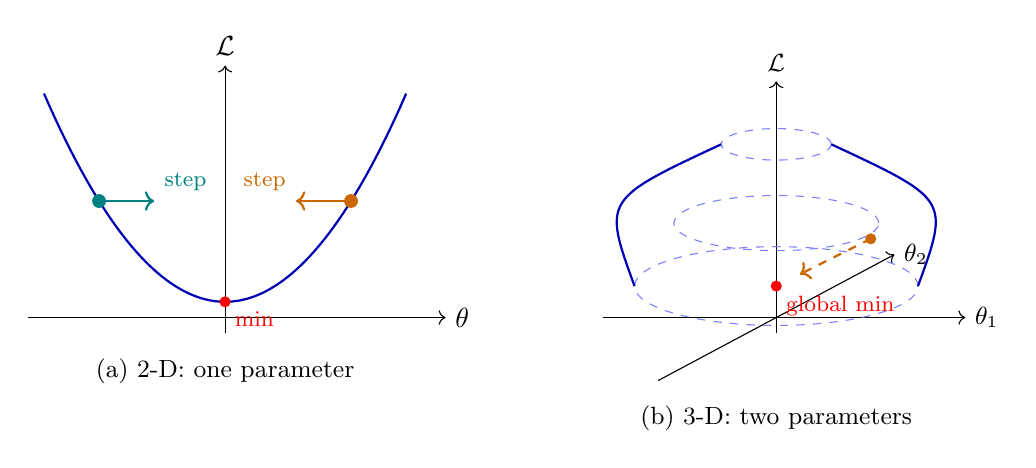
\begin{tikzpicture}
  %% ---- 2D loss curve (parabola-like) ----
  \begin{scope}[xshift=0cm]
    \draw[->] (-2.5,0) -- (2.8,0) node[right]{$\theta$};
    \draw[->] (0,-0.2) -- (0,3.2) node[above]{$\Loss$};
    %% parabola: y = (x)^2 * 0.5 + 0.2
    \draw[blue!70!black,thick,domain=-2.3:2.3,smooth,samples=60]
      plot (\x, {0.5*\x*\x + 0.2});
    %% minimum marker
    \fill[red] (0,0.2) circle (2pt) node[below right]{\footnotesize min};
    %% point on right slope
    \fill[orange!80!black] (1.6,{0.5*1.6*1.6+0.2}) circle (2.5pt);
    \draw[->,orange!80!black,thick]
      (1.6,{0.5*1.6*1.6+0.2}) -- +(-0.7,0)
      node[above left]{\footnotesize step};
    %% point on left slope
    \fill[teal] (-1.6,{0.5*1.6*1.6+0.2}) circle (2.5pt);
    \draw[->,teal,thick]
      (-1.6,{0.5*1.6*1.6+0.2}) -- +(0.7,0)
      node[above right]{\footnotesize step};
    \node[below] at (0,-0.4) {\small (a) 2-D: one parameter};
  \end{scope}

  %% ---- 3D bowl schematic ----
  \begin{scope}[xshift=7cm]
    %% axes
    \draw[->] (-2.2,0) -- (2.4,0) node[right]{\small$\theta_1$};
    \draw[->] (0,-0.2) -- (0,3.0) node[above]{\small$\Loss$};
    \draw[->] (-1.5,-0.8) -- (1.5,0.8) node[right]{\small$\theta_2$};
    %% ellipses to suggest a bowl
    \draw[blue!50,dashed] (0,0.4) ellipse (1.8cm and 0.5cm);
    \draw[blue!50,dashed] (0,1.2) ellipse (1.3cm and 0.35cm);
    \draw[blue!50,dashed] (0,2.2) ellipse (0.7cm and 0.2cm);
    %% bowl outline
    \draw[blue!70!black,thick]
      (-1.8,0.4) .. controls (-2.2,1.5) .. (-0.7,2.2);
    \draw[blue!70!black,thick]
      (1.8,0.4) .. controls (2.2,1.5) .. (0.7,2.2);
    %% minimum
    \fill[red] (0,0.4) circle (2pt) node[below right]{\footnotesize global min};
    %% gradient arrow
    \fill[orange!80!black] (1.2,1.0) circle (2pt);
    \draw[->,orange!80!black,thick,dashed] (1.2,1.0) -- (0.3,0.55);
    \node[below] at (0,-1.0) {\small (b) 3-D: two parameters};
  \end{scope}
\end{tikzpicture}
\caption{Loss landscape.
         (a) Convex 2-D curve: gradient descent steps (orange/teal arrows)
             always move toward the global minimum regardless of starting side.
         (b) Schematic 3-D bowl: the minimum occurs where all partial
             derivatives simultaneously equal zero.}
\label{fig:loss-landscape}
\end{figure}

\subsection{Multi-Dimensional Optimisation}

For a network with $n$ parameters the loss lives in an
$(n+1)$-dimensional space.
The minimum occurs when:
\begin{equation}
  \nabla_\Theta \Loss = \mathbf{0}
  \quad\Longleftrightarrow\quad
  \pderiv{\Loss}{\theta_i} = 0 \;\; \forall\, i = 1,\ldots,n.
  \label{eq:minimum-condition}
\end{equation}
Gradient descent iteratively approaches this point without requiring an
analytic solution of \cref{eq:minimum-condition}.

\begin{remark}
\label{rem:convex-vs-nonconvex}
For the squared-error loss used in this session, the loss landscape is
\emph{convex} with a unique global minimum (assuming fixed architecture and
data).
In practice, deep network loss landscapes are highly non-convex with many
local minima and saddle points.
However, empirical evidence shows that most local minima in deep networks
have similar loss values to the global minimum, and that gradient-based
methods find good solutions in practice.
\end{remark}

\subsection{The Role of Convergence}

\begin{definition}[Convergence]
\label{def:convergence}
Training is said to have \emph{converged} when parameter updates become
negligibly small:
\begin{equation}
  \|\theta^{(t+1)} - \theta^{(t)}\|
    = \eta\,\left\|\pderiv{\Loss}{\theta}\right\| < \varepsilon
  \label{eq:convergence}
\end{equation}
for a chosen tolerance $\varepsilon > 0$.
Equivalently, convergence can be declared when the loss ceases to decrease
significantly between iterations.
\end{definition}

% =============================================================================
\section{Learning Rate: Effects and Selection}
\label{sec:lr}
% =============================================================================

\subsection{Role of the Learning Rate}

The learning rate $\eta$ acts as a \emph{step-size multiplier}.
Together with the gradient, it determines how far the parameter moves in each
update.
Neither the gradient alone nor the learning rate alone is sufficient:
\begin{equation}
  \Delta\theta = -\eta\,\pderiv{\Loss}{\theta}.
  \label{eq:step}
\end{equation}

\subsection{Three Regimes}

\begin{table}[ht]
\centering
\caption{Effect of learning rate magnitude on training behaviour.}
\label{tab:lr-effects}
\begin{tabular}{p{2.5cm}p{4.5cm}p{5.5cm}}
\toprule
\textbf{Learning rate} & \textbf{Behaviour} & \textbf{Risk} \\
\midrule
Too small
  ($\eta \ll 1$) &
  Tiny steps; slow progress toward minimum. &
  Very slow convergence; may require millions of iterations. \\[6pt]
Moderate
  ($\eta \approx 0.01$) &
  Steady, stable descent toward minimum. &
  Best practical choice; may still require tuning. \\[6pt]
Too large
  ($\eta \gg 1$) &
  Overshoots the minimum; parameters jump to the opposite side. &
  Divergence or \emph{exploding gradients}; loss may increase. \\
\bottomrule
\end{tabular}
\end{table}

\begin{example}[Why $\eta = 10^{-4}$ was chosen in this session]
With gradients as large as 1413.12 (for $w_{11}$), a learning rate of
$\eta = 1$ would produce a parameter change of 1413 --- from $w_{11}=0.02$
to roughly $-1413$.
Using $\eta = 10^{-4}$ scales the largest step down to
$10^{-4} \times 1413 \approx 0.14$, a manageable change.
The instructor notes that the chosen learning rate is unusually small
precisely because the inputs $x_1=80$ and $x_2=8$ have very different scales.
The correct practice is to \emph{normalise inputs first}, then use a
moderate $\eta \approx 0.01$.
\end{example}

\begin{keyinsight}[title=Learning rate as speed control]
Think of the learning rate as a speed limit on the drive to the global
minimum.
If the speed is too low (small $\eta$), the journey takes too long.
If the speed is too high (large $\eta$), the driver overshoots the
destination and may end up on the opposite side.
A moderate speed allows reaching the destination reliably and in
reasonable time.
\end{keyinsight}

% =============================================================================
\section{Gradient Descent Variants}
\label{sec:gd-variants}
% =============================================================================

Once the gradient and update rule are understood for a single sample,
the question becomes: \emph{which data samples should drive each parameter
update?}
There are three standard answers.

\subsection{Batch Gradient Descent (BGD)}

Process \emph{all} $N$ training samples, accumulate the losses, then perform
one parameter update:
\begin{equation}
  \Loss_{\text{batch}} = \frac{1}{N}\sum_{i=1}^{N}\Loss(x^{(i)}, y^{(i)};\,\Theta),
  \label{eq:bgd-loss}
\end{equation}
\begin{equation}
  \theta \leftarrow \theta - \eta\,\pderiv{\Loss_{\text{batch}}}{\theta}.
  \label{eq:bgd-update}
\end{equation}

One pass through all $N$ samples plus one update is called one
\emph{epoch}.

\paragraph{Properties:}
\begin{itemize}[leftmargin=2em]
  \item Smooth, stable loss curve; gradient direction accurately reflects
        the entire dataset.
  \item Memory intensive: the entire dataset must fit in memory
        (or be streamed).
  \item Computationally expensive per update: $O(N)$ forward passes
        before any parameter change.
  \item Highly vectorisable; excellent GPU utilisation when $N$ is not
        too large.
\end{itemize}

\subsection{Stochastic Gradient Descent (SGD)}

Update parameters \emph{after every single sample}:
\begin{equation}
  \theta \leftarrow \theta - \eta\,\pderiv{\Loss(x^{(i)}, y^{(i)};\,\Theta)}{\theta}
  \quad \text{for each } i = 1, \ldots, N.
  \label{eq:sgd-update}
\end{equation}
In one epoch there are $N$ parameter updates.

\paragraph{Properties:}
\begin{itemize}[leftmargin=2em]
  \item Very fast per-update; parameters change after every single sample.
  \item High variance: the loss curve is noisy and zigzag because each
        sample provides only a partial view of the true gradient.
  \item Can escape shallow local minima due to noisy updates.
  \item Poor vectorisation: only one sample processed at a time.
  \item Convergence in terms of \emph{number of parameter updates} is fast,
        but wall-clock time may exceed BGD because of 1000$\times$ more
        gradient computations per epoch.
\end{itemize}

\subsection{Mini-Batch Gradient Descent (MBGD)}

Process $M$ samples (the \emph{mini-batch}) at a time:
\begin{equation}
  \Loss_{\text{mini}} = \frac{1}{M}\sum_{i \in \mathcal{B}}\Loss(x^{(i)}, y^{(i)};\,\Theta),
  \label{eq:mbgd-loss}
\end{equation}
\begin{equation}
  \theta \leftarrow \theta - \eta\,\pderiv{\Loss_{\text{mini}}}{\theta}.
  \label{eq:mbgd-update}
\end{equation}
With $N=100$ samples and $M=10$, there are 10 updates per epoch.

\paragraph{Properties:}
\begin{itemize}[leftmargin=2em]
  \item \textbf{Best of both worlds}: more stable than SGD, faster than BGD.
  \item GPU-friendly: batch size $M$ is chosen to fit in GPU memory.
  \item Typical values: $M \in \{16, 32, 64, 128, 256\}$.
  \item The \emph{de facto} standard in modern deep learning.
\end{itemize}

\subsection{Comparison Table}

\begin{table}[ht]
\centering
\caption{Comparison of gradient descent variants.
         $N$ = dataset size; $M$ = mini-batch size; $T$ = epochs.}
\label{tab:gd-comparison}
\begin{tabularx}{\linewidth}{lXXXX}
\toprule
\textbf{Variant} &
\textbf{Samples per update} &
\textbf{Updates per epoch} &
\textbf{Convergence} &
\textbf{Vectorisation} \\
\midrule
BGD  & $N$ (all) & 1         & Smooth, slow  & Excellent \\
SGD  & 1         & $N$       & Noisy, fast   & Poor      \\
MBGD & $M$       & $N/M$     & Balanced      & Good (GPU)\\
\bottomrule
\end{tabularx}
\end{table}

\subsection{Convergence Trajectories}

\begin{figure}[ht]
\centering
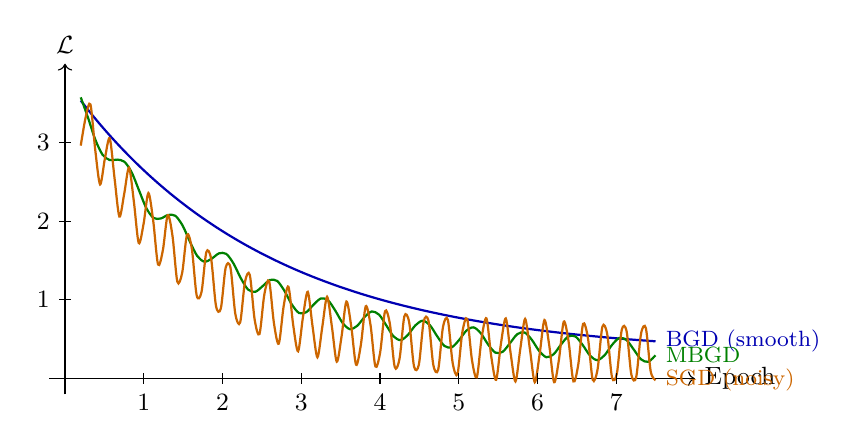
\begin{tikzpicture}[font=\small]
  \draw[->] (-0.2,0) -- (8,0) node[right]{Epoch};
  \draw[->] (0,-0.2) -- (0,4) node[above]{$\Loss$};

  %% BGD: smooth curve
  \draw[blue!70!black,thick,domain=0.2:7.5,smooth,samples=60]
    plot (\x, {3.5*exp(-0.4*\x)+0.3})
    node[right]{\footnotesize BGD (smooth)};

  %% MBGD: slightly noisy
  \draw[green!50!black,thick,domain=0.2:7.5,smooth,samples=80]
    plot (\x, {3.5*exp(-0.55*\x) + 0.3 + 0.15*sin(10*\x r)})
    node[right]{\footnotesize MBGD};

  %% SGD: very noisy
  \draw[orange!80!black,thick,domain=0.2:7.5,smooth,samples=120]
    plot (\x, {3.5*exp(-0.7*\x) + 0.3 + 0.4*sin(25*\x r)})
    node[right]{\footnotesize SGD (noisy)};

  %% axis ticks
  \foreach \x in {1,2,3,4,5,6,7}
    \draw (\x,2pt) -- (\x,-2pt) node[below]{\x};
  \foreach \y in {1,2,3}
    \draw (2pt,\y) -- (-2pt,\y) node[left]{\y};
\end{tikzpicture}
\caption{Schematic loss curves for the three gradient descent variants.
         BGD is smooth but slow to converge per epoch.
         SGD converges fastest in terms of parameter updates but is noisy.
         MBGD provides a practical balance.}
\label{fig:loss-curves}
\end{figure}

\begin{remark}
\label{rem:sgd-escape}
The noise in SGD is not always harmful: the random fluctuations can help
the optimiser escape shallow local minima.
This \emph{implicit regularisation} effect of SGD/MBGD is one reason why
small batch sizes are still used in practice even when larger batches would
fit in memory.
\end{remark}

% =============================================================================
\section{PyTorch Implementation Notes}
\label{sec:pytorch}
% =============================================================================

The session includes a live coding demonstration.
The key PyTorch patterns are outlined below.

\subsection{Data Generation}

The instructor creates a synthetic 500-sample IQ/CGPA$\to$LPA dataset:

\begin{verbatim}
import torch
N = 500
torch.manual_seed(42)
IQ   = torch.randint(50, 130, (N, 1)).float()
CGPA = 5 + 5 * torch.rand(N, 1)
X = torch.cat([IQ, CGPA], dim=1)   # shape: (500, 2)
Y = 0.1*IQ + 0.5*CGPA + 0.01*torch.randn(N,1)
\end{verbatim}

\subsection{Manual Parameter Initialisation}

Nine parameters are created with \texttt{requires\_grad=True} so that
PyTorch's autograd engine can compute their gradients automatically:

\begin{verbatim}
params = [
    torch.tensor([[0.02]], requires_grad=True),  # w11
    torch.tensor([[0.50]], requires_grad=True),  # w12
    ...  # (all 9 parameters)
]
\end{verbatim}

\subsection{Training Loop Skeleton}

\begin{verbatim}
lr = 1e-4
for epoch in range(200):
    # Forward pass
    z1 = X[:,0:1]*params[0] + X[:,1:2]*params[1] + params[4]
    h1 = torch.relu(z1)
    z2 = X[:,0:1]*params[2] + X[:,1:2]*params[3] + params[5]
    h2 = torch.relu(z2)
    yhat = params[6]*h1 + params[7]*h2 + params[8]
    loss = ((yhat - Y)**2).mean()

    # Backward pass
    loss.backward()

    # Parameter update (manual)
    with torch.no_grad():
        for p in params:
            p -= lr * p.grad
            p.grad.zero_()
\end{verbatim}

\begin{keyinsight}[title=Gradient zeroing]
The call \texttt{p.grad.zero\_()} after each update is mandatory.
PyTorch accumulates (adds) gradients by default.
Without zeroing, gradient from iteration $t-1$ would be added to the
gradient at iteration $t$, corrupting the update.
\end{keyinsight}

\subsection{Switching Between Gradient Descent Variants}

\begin{table}[ht]
\centering
\caption{How to implement each GD variant in PyTorch by adjusting the
         \texttt{DataLoader} batch size.}
\label{tab:pytorch-gd}
\begin{tabular}{lll}
\toprule
\textbf{Variant} & \textbf{DataLoader setting} & \textbf{Updates per epoch} \\
\midrule
BGD  & \texttt{batch\_size=N} (full dataset) & 1 \\
SGD  & \texttt{batch\_size=1}                & $N$ \\
MBGD & \texttt{batch\_size=32} (or 64, 128)  & $\lceil N/32 \rceil$ \\
\bottomrule
\end{tabular}
\end{table}

% =============================================================================
\section{Summary and Conclusions}
\label{sec:summary}
% =============================================================================

\subsection{Session Recap}

Session~07 provided a fully numerical end-to-end demonstration of the
backpropagation algorithm on the canonical 2-2-1 network, and established the
conceptual framework needed for training deeper networks.
The key steps were:

\begin{enumerate}[leftmargin=2em,label=\textbf{\arabic*.}]
  \item \textbf{Forward pass} ($x_1=80$, $x_2=8$, $y=3$): produced
        $\yhat = 10.36$, $\Loss = 54.17$.
  \item \textbf{Backward pass}: computed all 9 gradients using the chain
        rule.  The largest gradient ($\pderiv{\Loss}{w_{11}} = 1413.12$) arose
        because $x_1 = 80$ amplifies every factor in the chain-rule product.
  \item \textbf{Parameter update} ($\eta = 10^{-4}$): all 9 parameters
        updated simultaneously; new loss $= 4.006$ --- a 92.6\% reduction in
        one step.
  \item \textbf{Gradient concept}: gradient is slope; gradient descent
        subtracts a scaled slope, always moving downhill regardless of which
        side of the minimum the current point is on.
  \item \textbf{Gradient descent variants}: BGD (stable, slow), SGD (noisy,
        fast), MBGD (balanced, GPU-friendly).
\end{enumerate}

\subsection{Key Takeaways}

\begin{table}[ht]
\centering
\caption{Core messages from Session~07 and their implications for practice.}
\label{tab:takeaways}
\begin{tabularx}{\linewidth}{p{4cm}X}
\toprule
\textbf{Concept} & \textbf{Practical implication} \\
\midrule
Chain rule drives backprop &
  Every parameter is reachable via the chain rule; no special treatment
  needed for deeply buried weights. \\[4pt]
Input scale $\to$ gradient scale &
  Normalise features before training to prevent pathologically large
  gradients for weights connected to large-valued inputs. \\[4pt]
Learning rate controls step size &
  Tune $\eta$; neither too large (diverge) nor too small (slow).
  Common starting points: $0.01$--$0.001$. \\[4pt]
Dead ReLU after large steps &
  Overshooting can kill ReLU neurons.
  Use proper weight initialisation and gradient clipping. \\[4pt]
MBGD is the default &
  Mini-batch gradient descent with batch size 32--256 balances
  speed, stability, and GPU memory. \\
\bottomrule
\end{tabularx}
\end{table}

\subsection{Looking Ahead}

The next sessions will build on these foundations to cover:
\begin{itemize}[leftmargin=2em]
  \item The \textbf{vanishing gradient problem} and how it arises when
        deep networks use sigmoid or tanh activations.
  \item Solutions: ReLU family, batch normalisation, residual connections.
  \item The \texttt{torch.nn} module for building networks without manual
        parameter management.
  \item The \texttt{torch.optim} module, which encapsulates the update rule
        and supports advanced optimisers (Adam, RMSProp, Momentum SGD).
  \item Convolutional Neural Networks (CNN), Recurrent Neural Networks
        (RNN), and Long Short-Term Memory (LSTM) networks, where the same
        chain-rule mechanics apply.
\end{itemize}

\begin{keyinsight}[title=Universality of backpropagation]
Every concept introduced in this session --- chain rule, gradient
computation, learning rate, mini-batch processing --- applies unchanged to
CNN, RNN, and Transformer architectures.
The only difference is the \emph{form} of the forward-pass equations;
the backward pass machinery is always the same.
\end{keyinsight}

\clearpage

\end{document}
